% #############################################################################
% This is Chapter 4
% !TEX root = ../main.tex
% #############################################################################
\fancychapter{Numerical Results}
% \cleardoublepage
\label{chap:implement}

In this chapter, the results found for the Dirac operator with infinite mass boundary conditions and the transmission problem are presented. For each problem, a numerical validation of the method is presented, in cases where closed-form solutions are available. Every simulation was implemented in Python 3.10.

\section{Dirac equation simulations}\label{dirac_equation_simulations}

Recall the system of equations given in \eqref{dirac}
\begin{equation}\label{chapt_num_dirac_eq}
    \begin{bmatrix}
        m & -i(\partial_1 - i \partial_2)\\
        -i(\partial_1 + i \partial_2) & -m
    \end{bmatrix}
    \begin{bmatrix}
        u_1(x)\\
        u_2(x)
    \end{bmatrix}
    =\lambda
    \begin{bmatrix}
    u_1(x)\\
    u_2(x)
    \end{bmatrix},
\end{equation}
which can be reduced to the Helmholtz equation with Cauchy-Riemann oblique boundary conditions
\begin{equation*}
    \begin{cases}
        &-\Delta u_1 = (\lambda^2 - m^2)u_1, \; \text{ in } \Omega\\
        & i (\partial_1 + i\partial_2)u_1 + (\lambda + m)i(n_1 + i n_2)u_1 = 0, \; \text{ on } \Gamma,
    \end{cases}      
\end{equation*}
where \(\Gamma = \partial\Omega\) as usual, and the function \(u_2\) depends on the function \(u_1\) through the following equality
\[
    u_2 = \frac{-i (\partial_1 + i\partial_2)u_1}{\lambda + m}.    
\]
\subsection{Numerical validation of the method}

In order to validate the MFS for the Dirac equation with infinite mass boundary conditions, we start by testing it for the unit disk. If \(m=0\), then as stated in Proposition \ref{dirac_properties}, the first eigenvalue of problem \eqref{chapt_num_dirac_eq} is \(\lambda_1(\mathbb{D})= 1.434695650819\), obtained as the smallest positive solution of the equation
\[
    J_0(\lambda_1(\mathbb{D})) = J_1(\lambda_1(\mathbb{D})).
\]

In the numerical simulations presented below, 158 inner collocation points for the Subspace Angle Technique (see section \ref{sat_appendix} in Appendix \ref{chapter:appendixB}) were considered\footnote{In Figure \ref{dirak_disk_col_m0}, the inner collocation points were chosen in a lattice. However, one can place these points freely, in a lattice, or randomly. In fact, in some simulations, the inner points were placed using pseudo-random Halton sequences \cite{halton1964algorithm}.} and the number of source points \(N\) was always half of the number of boundary points. Figure \ref{dirak_disk_col_m0} shows the configuration used. The method described at the end of the subchapter \ref{density_proofs_section}, below Remark \ref{density_remark_general_bc_and_hilbert}, was used to place the source points, with \(\eta=0.5\). 

\begin{figure}[!htb]
    \centering
    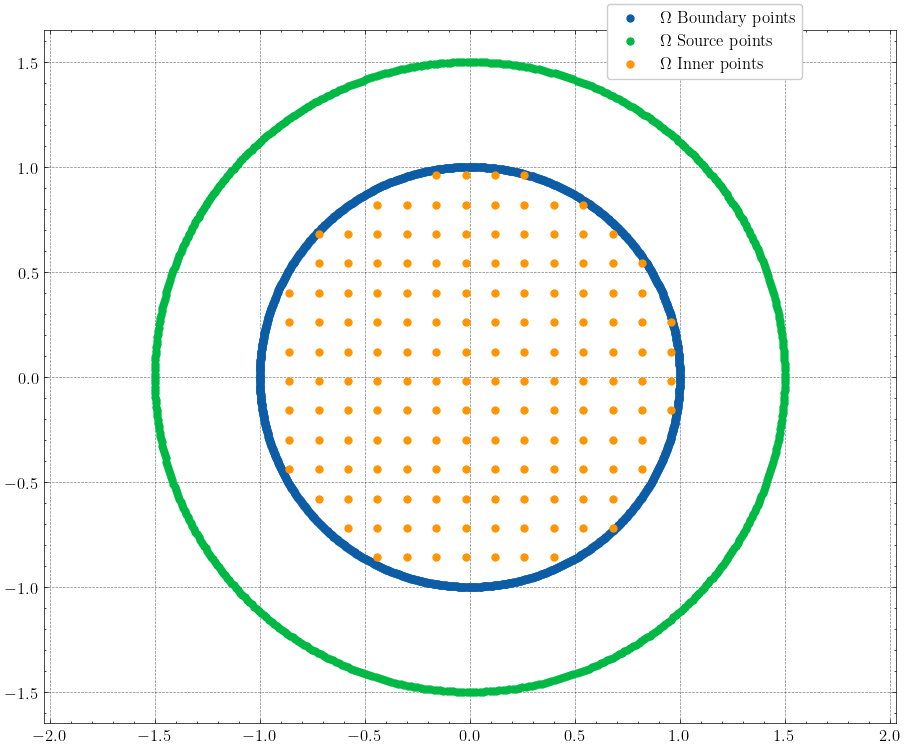
\includegraphics[width=0.5\linewidth]{Images/Dirac/circle_m_0_col_points_158_inner_eta_05.png}
    \captionof{figure}{Configuration of the boundary, source, and inner points. The number of boundary collocation points used is 1200.}
    \label{dirak_disk_col_m0}
\end{figure}

While in the other numerical simulations more eigenvalues are studied, in Table \ref{tab:eigenvalues_disk_val} only the first three eigenvalues are shown for the sake of brevity.

\begin{table}[htbp]
    \centering
    \begin{tabular}{cccc}
        \toprule
        \textbf{Eigenvalues} & \textbf{N=1200} & \textbf{N=1000} & \textbf{N=800} \\
        \midrule
        \(\tilde{\lambda}_1(\mathbb{D})\) & $1.4346956515$ & $1.4346956481$ & $1.4346956367$ \\
        \(\tilde{\lambda}_2(\mathbb{D})\) & $2.6298741163$ & $2.6298741147$ & $2.6298741276$ \\
        \(\tilde{\lambda}_3(\mathbb{D})\) & $3.1128644920$ & $3.1128645083$ & $3.1128645008$ \\
        \midrule
        \textbf{Absolute error: } \(\abs{\lambda_1(\mathbb{D}) - \tilde{\lambda}_1(\mathbb{D})}\) & $6,877\times 10^{-10}$ & $2,693\times 10^{-9}$ & $1,413\times 10^{-8}$ \\
        \bottomrule
    \end{tabular}
    \caption{Eigenvalues for different values of \(N\) and the measured absolute error.}
    \label{tab:eigenvalues_disk_val}
\end{table}

The results obtained using the bracketing algorithm \ref{direct_bracketing_algorithm} are plotted in Figure \ref{dirac_disk_alg_m0}. For future reference, the first eigenfunction on the disk with \(m=0\) is shown in Figure \ref{dirac_disk_plots_m0}, with the real and imaginary parts of the spinors \(u_1\) and \(u_2\) plotted. The functions in the plots are also normalized, i.e., \(\norm*{\mathbf{u}}_{L^2(\mathbb{D})}=1\).

\begin{figure}[!htb]
    \centering
    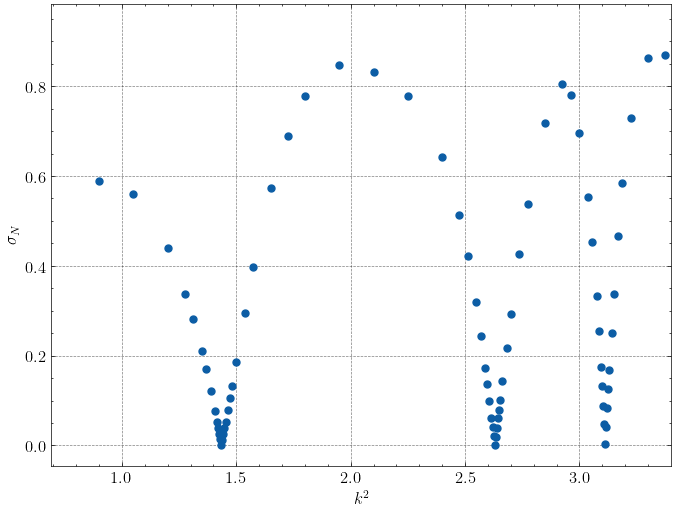
\includegraphics[width=0.5\linewidth]{Images/Dirac/circle_m_0_alg_points_158_inner_eta_05.png}
    \captionof{figure}{Results obtaiend by the direct search algorithm for the first three eigenvalues of the disk with \(m=0\). In practice, more accurate approximations are achieved when smaller values of the smallest singular value \(\sigma_N\) of the matrix \(Q(k)\) (studied in section \ref{sat_appendix}) are identified at each minimum.}
    \label{dirac_disk_alg_m0}
\end{figure}

\begin{figure}[!htb]
    \centering
    \begin{minipage}[b]{0.45\textwidth}
        \centering
        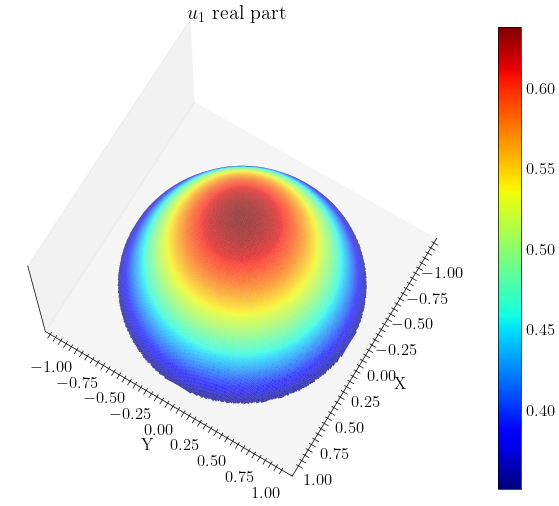
\includegraphics[width=0.8\textwidth]{Images/Dirac/circle_m_0_u1_re_points_158_inner_eta_05.png}
%\caption{Network 1}
    \end{minipage}
    \hfill
    \begin{minipage}[b]{0.45\textwidth}
        \centering
        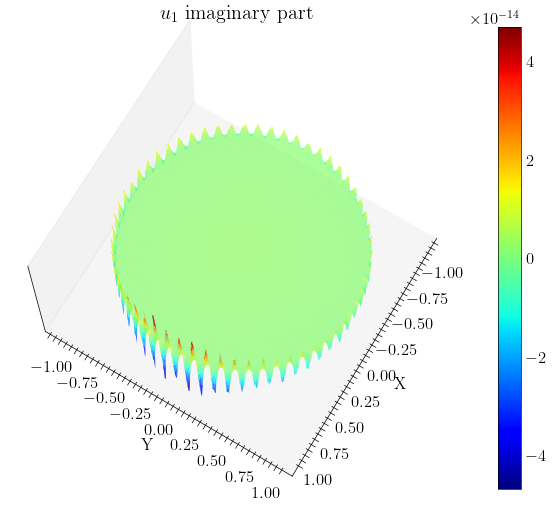
\includegraphics[width=0.8\textwidth]{Images/Dirac/circle_m_0_u1_im_points_158_inner_eta_05.png}
%\caption{Network 2}
    \end{minipage}

    \vspace{0.5cm}

    \begin{minipage}[b]{0.45\textwidth}
        \centering
        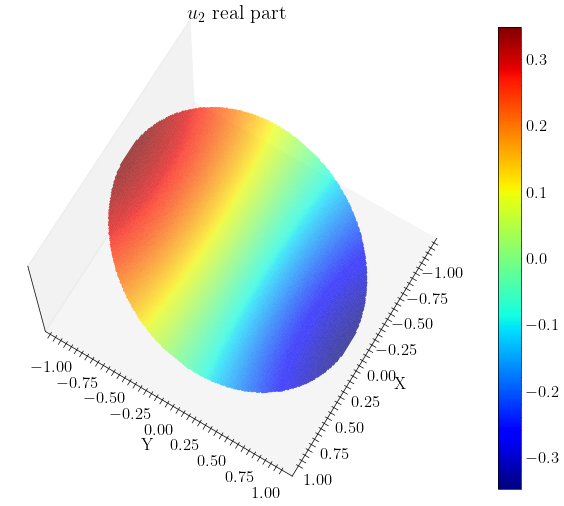
\includegraphics[width=0.8\textwidth]{Images/Dirac/circle_m_0_u2_re_points_158_inner_eta_05.png}
%\caption{Network 3}
    \end{minipage}
    \hfill
    \begin{minipage}[b]{0.45\textwidth}
        \centering
        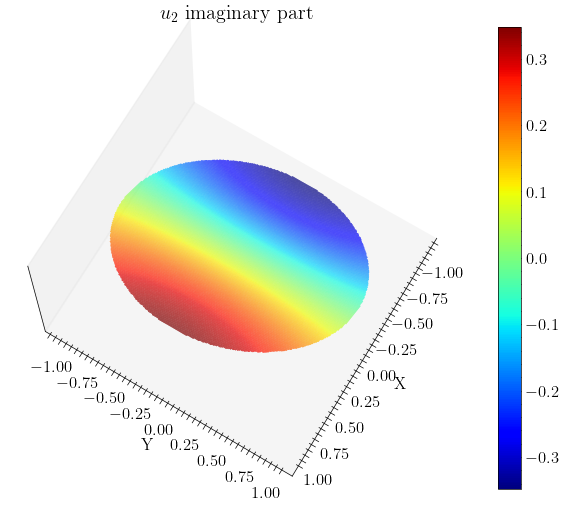
\includegraphics[width=0.8\textwidth]{Images/Dirac/circle_m_0_u2_im_points_158_inner_eta_05.png}
%\caption{Network 4}
    \end{minipage}
    \caption{Plots of the real and imaginary parts of \(u_1\) and \(u_2\) of the first eigenfunction \(\mathbf{u}=\begin{bmatrix} u_1\\ u_2 \end{bmatrix}\). Observe that the imaginary part of \(u_1\) is zero and the artifacts presented are due to precision lost.}
    \label{dirac_disk_plots_m0}
\end{figure}



\subsection{Quadrilateral results}\label{chap_numerics_dirac_quad_section}

In this subsection, several numerical results regarding quadrilateral polygons are shown and discussed. First, numerical evidence for the Conjecture \ref{david_conjectures} is presented both for \(m=1\) and \(m=5\). Then, some simulations suggest that the conjectured Ashbaugh-Benguria Theorem \ref{conjecture_benguria} also holds for the Dirac operator with infinite-mass boundary conditions. Finally, we also show that some disagreement between the spectrum of the Laplace and Dirac operators is already evident for the third eigenvalue, whose optimal shape is not the disk for somes values of \(m\), contrary to what is conjectured for the Laplacian (which is still an open problem).

Consider a rectangle with a width \(a \geq 1\) and unitary area, where the sides are \(a\) and \(\frac{1}{a}\). Figures \ref{eigenvalues_rectangle_width_m_1} and \ref{eigenvalues_rectangle_width_m_5} illustrate the behavior of the first 5 eigenvalues for \(m=1\) and \(m=5\), respectively. Several interesting observations can be made:

\begin{enumerate}
  \item \label{dirac_sim_quad_point_1} The behavior of the spectrum remains qualitatively consistent for different values of \(m\). Significantly, as \(m\) increases, the eigenvalues approach \(m\) with a diminishing gap, while remaining greater than \(m\). While this trend is discernible already in Figures \ref{eigenvalues_rectangle_width_m_1} and \ref{eigenvalues_rectangle_width_m_5}, it becomes more apparent as \(m\) takes on even larger values. It is important to point out that the third eigenvalue is not globally minimized in the square for \(m=1\), but for some rectangle with width \(a \approx 2.2\). However, this does not appear to hold for any mass \(m \geq 0\) but only for some values of \(m \leq m_{\text{crit}}\), where \(1 \leq m_{\text{crit}} \leq 5\), i.e., for any mass \(m \leq m_{\text{crit}}\) the global minimizer of the third eigenvalue is some (non-square) rectangle.
  
  \item \label{dirac_sim_quad_point_2}  Starting from the third eigenvalue and beyond, certain spikes become evident in the plot. These spikes correspond to rectangular domains where the eigenvalue has a multiplicity of two. For instance, between the values 1 and 1.5, the third and fourth eigenvalues appear to coincide. This behavior becomes more frequent as the order of the eigenvalues increases.
  %However, only multiplicity 2 is observed which is not consistent with the behavior seen in the Laplace operator, where multiplicity 3 is already achieved in the third eigenvalue and only the first eigenvalue is simple;
  
  \item \label{dirac_sim_quad_point_3} By increasing the value of the parameter \(a\), a linear growth in the eigenvalues magnitude is observed, with no change in their multiplicity. As \(a\) increases, the eigenvalues draw closer to each other, which is an expected outcome. This behavior arises as the rectangular domain transforms into an unbounded line, giving rise to a continuous spectrum.
\end{enumerate}

\begin{figure}[!htb]
    \centering
    \begin{minipage}{.5\textwidth}
      \centering
      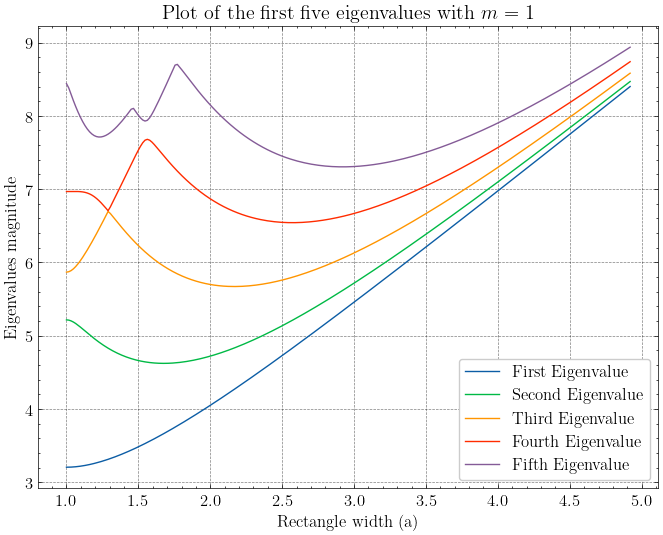
\includegraphics[width=\linewidth]{Images/Dirac/quad/eigenvalues_rectangle_width_m_1.png}
      \captionsetup{width=0.9\linewidth} % Adjust the width of the caption
      \captionof{figure}{Behavior of the first five eigenvalues for rectangles with unit area, width \(a\) and \(m=1\).}
      \label{eigenvalues_rectangle_width_m_1}
    \end{minipage}%
    %\hspace{0.5cm} % Add some horizontal space between the figures
    \begin{minipage}{.5\textwidth}
      \centering
      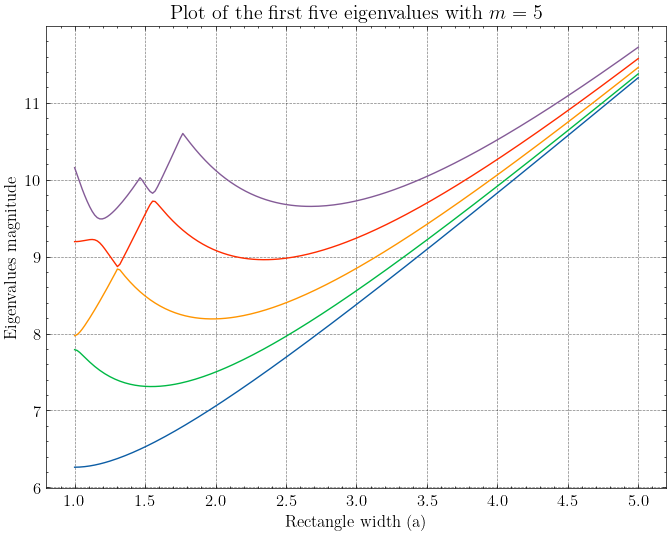
\includegraphics[width=1\linewidth]{Images/Dirac/quad/eigenvalues_rectangle_width_m_5.png}
      \captionsetup{width=0.9\linewidth} % Adjust the width of the caption
      \captionof{figure}{Behavior of the first five eigenvalues for rectangles with unit area, width \(a\) and \(m=5\).}
      \label{eigenvalues_rectangle_width_m_5}
    \end{minipage}
\end{figure}

In Figures \ref{eigenvalues_rectangle_perimeter_width_m_1} and \ref{eigenvalues_rectangle_perimeter_width_m_5} the results with fixed perimeter \(L=4\) are shown. While Conjecture \ref{david_conjectures} is stated for \(a \in (0, 2)\) it is enough to consider \(a \in (0, 1)\) given the symmetry of the problem and the fact that the perimeter is equal to 4. Note that the area of the rectangle may change when the perimeter is fixed and the rectangle width varies. The conclusions and remarks presented in points \ref{dirac_sim_quad_point_1} and \ref{dirac_sim_quad_point_2} for rectangles with fixed area are still valid. In this case, point \ref{dirac_sim_quad_point_3} holds when \(a\) approaches zero.

\begin{figure}[!htb]
    \centering
    \begin{minipage}{.5\textwidth}
      \centering
      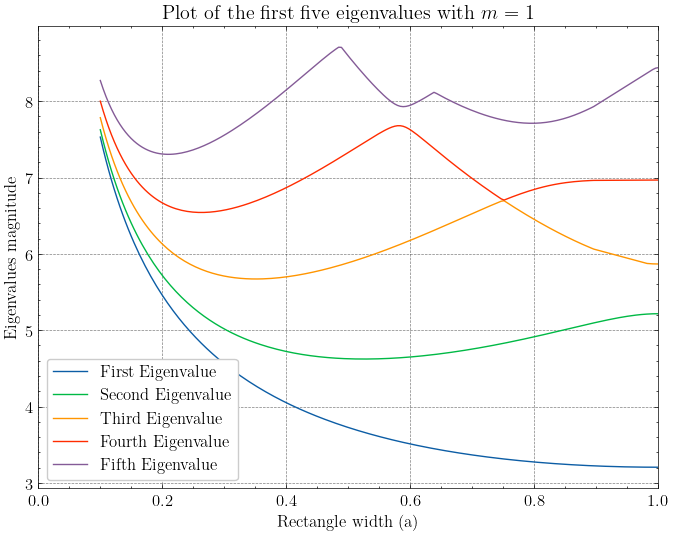
\includegraphics[width=\linewidth]{Images/Dirac/quad/eigenvalues_rectangle_perimeter_width_m_1.png}
      \captionsetup{width=0.9\linewidth} % Adjust the width of the caption
      \captionof{figure}{Behavior of the first five eigenvalues for rectangles with perimeter \(L=4\), width \(a\) and \(m=1\).}
      \label{eigenvalues_rectangle_perimeter_width_m_1}
    \end{minipage}%
    %\hspace{0.5cm} % Add some horizontal space between the figures
    \begin{minipage}{.5\textwidth}
      \centering
      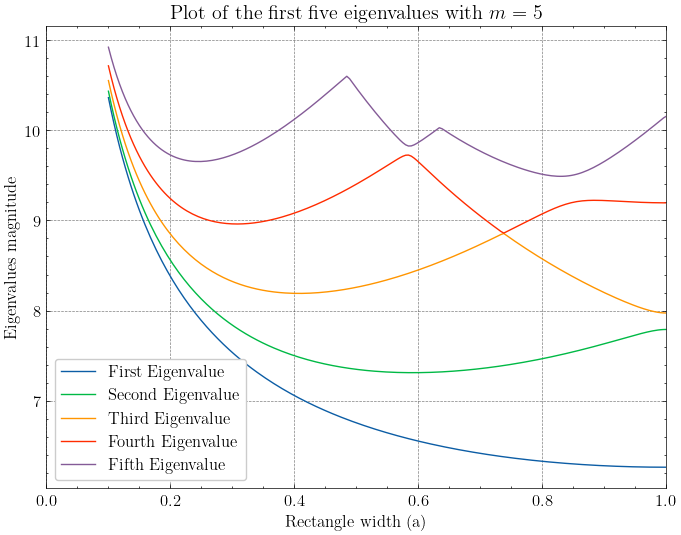
\includegraphics[width=1\linewidth]{Images/Dirac/quad/eigenvalues_rectangle_perimeter_width_m_5.png}
      \captionsetup{width=0.9\linewidth} % Adjust the width of the caption
      \captionof{figure}{Behavior of the first five eigenvalues for rectangles with perimeter \(L=4\), width \(a\) and \(m=5\).}
      \label{eigenvalues_rectangle_perimeter_width_m_5}
    \end{minipage}
\end{figure}

Given the results for rectangles with fixed area or perimeter, it is possible to state that the Conjecture \ref{david_conjectures} should hold, although it is not possible to ascertain that the results presented here hold for every \(m\) (as we saw before, the value of \(m\) has some discernible influence on the spectrum, which can already be seen for the third eigenvalue, although no difference was found for the first and second eigenvalues). In any case, it is known that the eigenvalues are continuous with domain perturbations (here these perturbations can be seen as stretching the rectangles), exactly what has been found in these numerical simulations.

To finish this subsection, we present the results for general quadrilaterals for \(m=1\). Since no (practical) parameterization can describe every quadrilateral, we have resorted to a random sampling of quadrilaterals and studied the results against rectangles and rhombi. Figure \ref{dirac_first_three_eigenvalues_quad_m_1} presents the results of the numerical simulations. For the third eigenvalue, it is already possible to find some domains whose third eigenvalue is smaller than the eigenvalue of the unit disk. In Figures \ref{dirac_benguria_quad} and \ref{dirac_generalized_benguria_quad} the ratio between the first eigenvalues is studied, and the version of the Ashbaugh-Benguria presented in Theorem \ref{conjecture_benguria} appears to hold.

\begin{figure}[!htb]
    \centering
    \begin{minipage}[c]{0.8\textwidth}
        \centering
        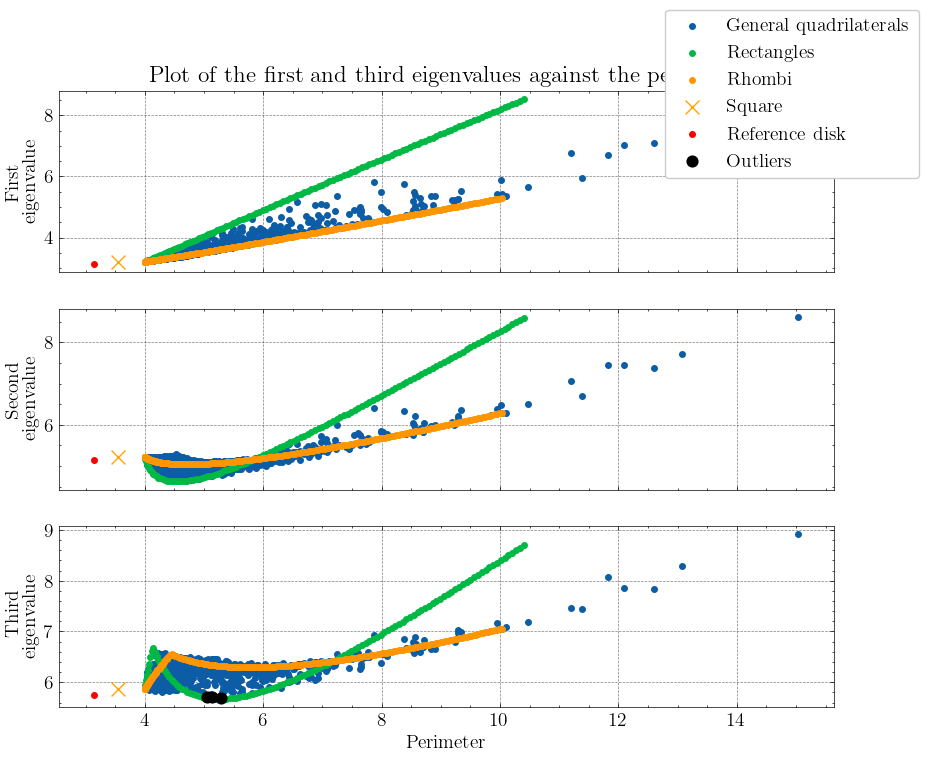
\includegraphics[width=0.8\textwidth]{Images/Dirac/quad/first_three_eigenvalues_quad_m_1.png}
        \caption{Plot of the first three eigenvalues against the perimeter for \(m=1\) for quadrilaterals. The ``outliers'' marked in black represent the domains in which the third eigenvalue is smaller than the third eigenvalue of the disk.}
        \label{dirac_first_three_eigenvalues_quad_m_1}
    \end{minipage}

    \vspace{0.5cm}

    \begin{minipage}[c]{0.45\textwidth}
        \centering
        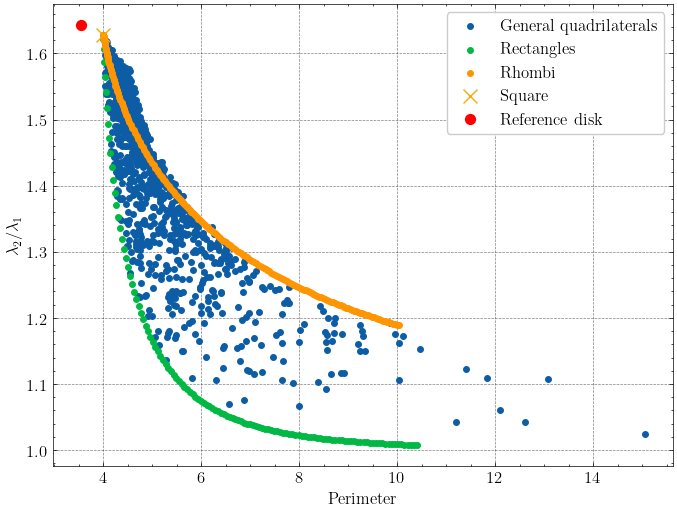
\includegraphics[width=\textwidth]{Images/Dirac/quad/benguria_quad.png}
        \captionsetup{width=0.8\linewidth} % Adjust the width of the caption
        \caption{Ratio between the first two eigenvalues \(\frac{\lambda_2}{\lambda_1}\) plotted against the perimeter for \(m=1\) for quadrilaterals, as in Figure \ref{dirac_first_three_eigenvalues_quad_m_1}.}
        \label{dirac_benguria_quad}
    \end{minipage}
    \hfill
    \begin{minipage}[c]{0.45\textwidth}
        \centering
        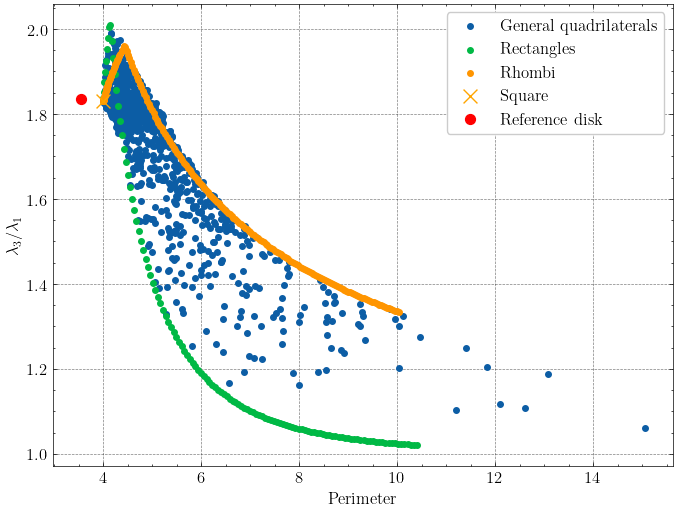
\includegraphics[width=\textwidth]{Images/Dirac/quad/generalized_benguria_quad.png}
        \captionsetup{width=0.8\linewidth} % Adjust the width of the caption
        \caption{Ratio between the third and first eigenvalues \(\frac{\lambda_3}{\lambda_1}\) plotted against the perimeter for \(m=1\) for quadrilaterals, as in Figure \ref{dirac_first_three_eigenvalues_quad_m_1}.}
        \label{dirac_generalized_benguria_quad}
    \end{minipage}
    \vspace{0.5cm}
\end{figure}

\subsection{Results for triangles and general polygons}\label{chap_numerics_dirac_triangles_section}

In this subsection, we tackle the Conjectures \ref{triangle_conjectures} stated in \cite{vu2023spectral}. At the end of the subsection, numerical evidence for Conjecture \ref{polya_szego_conjecture_dirac} is also presented. Instead of considering random triangles, this study can be done systematically given that, up to a congruence, three parameters completely define every triangle. The approach presented here is based on the work of Antunes and Freitas \cite{antunes2011inverse}. Consider the region \(R\) defined by
\[
    R = \{(x, y) \in \mathbb{R}^2: x \geq 0, y > 0, (x+1)^2 + y^2 \leq 4\},
\]
and its piecewise boundary \(\partial R = \Gamma_0 \cup \Gamma_1 \cup \Gamma_2\), where
\begin{align*}
    \Gamma_0 &= \{(x,y) \in \mathbb{R}^2: 0 \leq x \leq 1, y=0\}\\
    \Gamma_1 &= \{(x,y) \in \mathbb{R}^2: 0 \leq x < 1, y=\sqrt{4-(x+1)^2}\}\\
    \Gamma_2 &= \{(x,y) \in \mathbb{R}^2: x=0, 0 < y < \sqrt{3}\}.
\end{align*}
A triangle \(T\) is said to be \textit{admissible} if its basis vertices are \((0, 0)\) and \((1, 0)\), and the third vertex coordinates\footnote{Of course, one does not need to impose such constraints on the triangle: as said before, every triangle is unique up to congruence. Here, we just emphasize that it is enough to consider triangles in region \(R\). Observe that this is just a way to exhaust numerically all possible triangles up to a congruence.} are \((x,y)\) such that \((x,y) \in \overline{R}\). An isosceles triangle \(T\) is said to be \textit{subequilateral} if \((x, y) \in \Gamma_1\) with aperture less
than \(\frac{\pi}{3}\), and \textit{superequilateral} with aperture greater
than \(\frac{\pi}{3}\) such that \((x, y) \in \Gamma_2\); if \((x, y) = (0, \sqrt{3})\) then it is equilateral (obviously). The plot of the region \(R\) and its boundary \(\partial R\) is in Figure \ref{dirac_triangle_model}.

\begin{figure}[!htb]
    \centering
    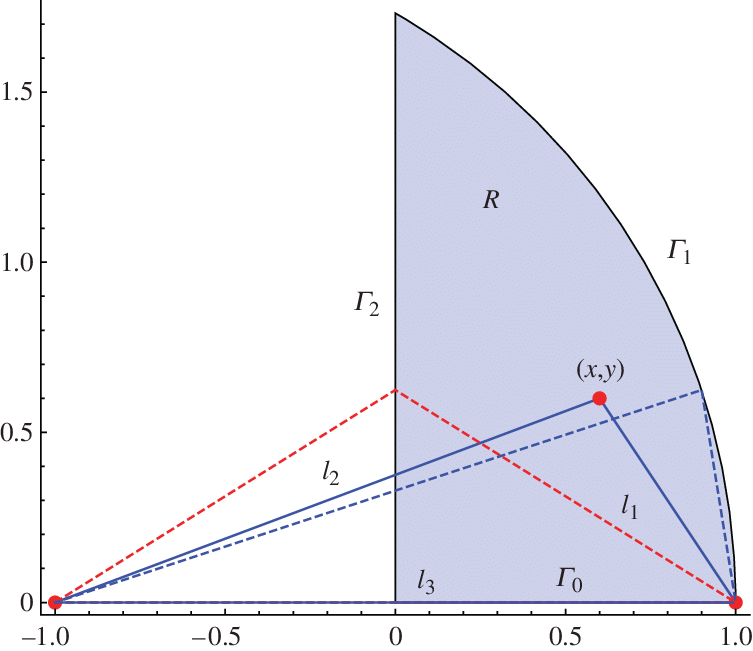
\includegraphics[width=0.5\linewidth]{Images/Dirac/model_triangle.png}
    \captionof{figure}{Configuration space of the admissible triangles. The dashed red line shows a subequilateral triangle; the dashed blue line a superequilateral triangle.}
    \label{dirac_triangle_model}
\end{figure}

In Figure \ref{dirac_smooth_first_eigenvalues}, we provide numerical evidence supporting Conjecture \ref{triangle_conjectures} with \(m=1\). It's noteworthy how the eigenvalues of the superequilateral and subequilateral triangles define a (very thin) region encompassing all other triangles with \((x, y)\) vertices in \(R\). Figure \ref{dirac_triangle_benguria} numerically corroborates a version of the Ashbaugh-Benguria (see Conjecture 3.2.6) Theorem
(see to Conjecture \ref{conjecture_benguria}). Additionally, in Figure \ref{dirac_triangle_3d_lambda1}, we present a 3D plot of the first eigenvalue for each admissible triangle against the vertex coordinates \((x,y)\) within \(\overline{R}\). Finally, Figure \ref{dirac_triangle_model_perimeter} also showcases the first three eigenvalues for triangles with a fixed perimeter \(L = 15\). This unconventional value was chosen due to the diminutive size of unit perimeter triangles, making the method implementation more challenging and prone to numerical errors. For example, for a very small triangle the distance between a boundary point \(x_i\) and a source point \(y_j\) is very small and \(\abs{x_i-y_j} \approx 0\) which implies that \(\abs{\Phi_k(\abs{x_i-yj})}\) is a very large value, since the fundamental solution explodes in the origin, negatively impacting the condition number.

In a manner similar to the conjecture regarding triangles with fixed area, the conjecture concerning triangles with fixed perimeter also seems to hold. Furthermore, it's worth noting that equilateral triangles minimize both the second and third eigenvalues.

\begin{figure}[!htb]
    \centering
    \begin{minipage}[c]{0.8\textwidth}
        \centering
        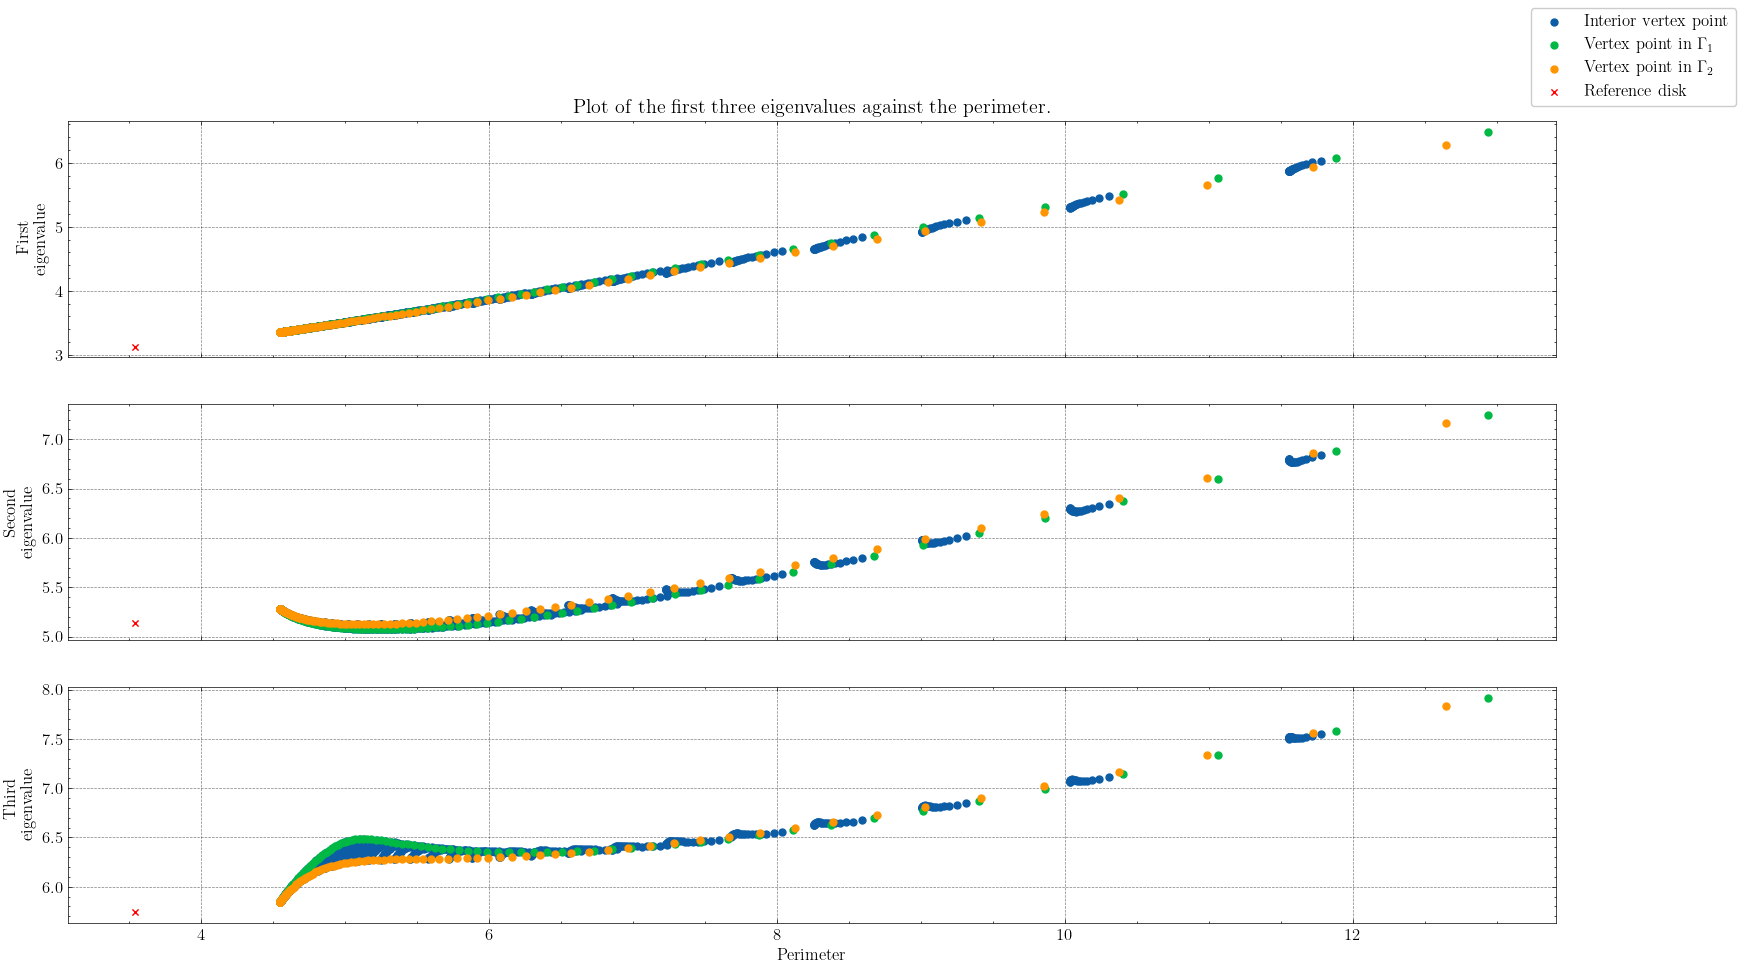
\includegraphics[width=\textwidth]{Images/Dirac/triangles/triangle_first_eigenvalues.png}
        \caption{Plot of the first three eigenvalues against the perimeter for triangular domains.}
        \label{dirac_smooth_first_eigenvalues}
    \end{minipage}

    \vspace{0.5cm}

    \begin{minipage}[c]{0.41\textwidth}
        \centering
        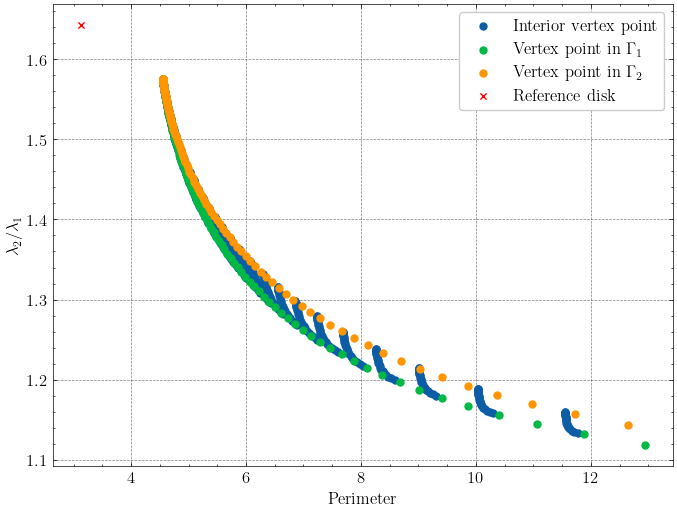
\includegraphics[width=\textwidth]{Images/Dirac/triangles/triangle_benguria.png}
        \captionsetup{width=0.9\linewidth} % Adjust the width of the caption
        \caption{Ratio between the first two eigenvalues \(\frac{\lambda_2}{\lambda_1}\) for triangular domains.}
        \label{dirac_triangle_benguria}
    \end{minipage}
    \hfill
    \begin{minipage}[c]{0.49\textwidth}
        \centering
        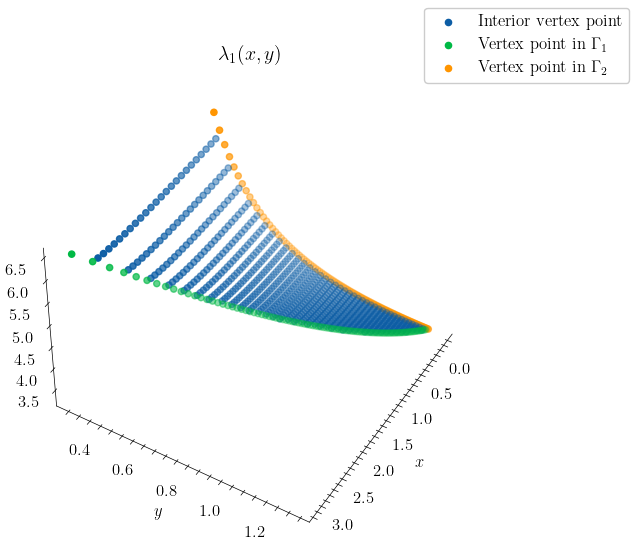
\includegraphics[width=\textwidth]{Images/Dirac/triangles/triangle_3d_lambda1.png}
        \captionsetup{width=0.9\linewidth} % Adjust the width of the caption
        \caption{Plot of the first eigenvalue \(\lambda_1(x,y)\) for each sample point \((x,y) \in R\) for triangular domains.}
        \label{dirac_triangle_3d_lambda1}
    \end{minipage}
    \vspace{0.5cm}
\end{figure}

\begin{figure}[!htb]
    \centering
    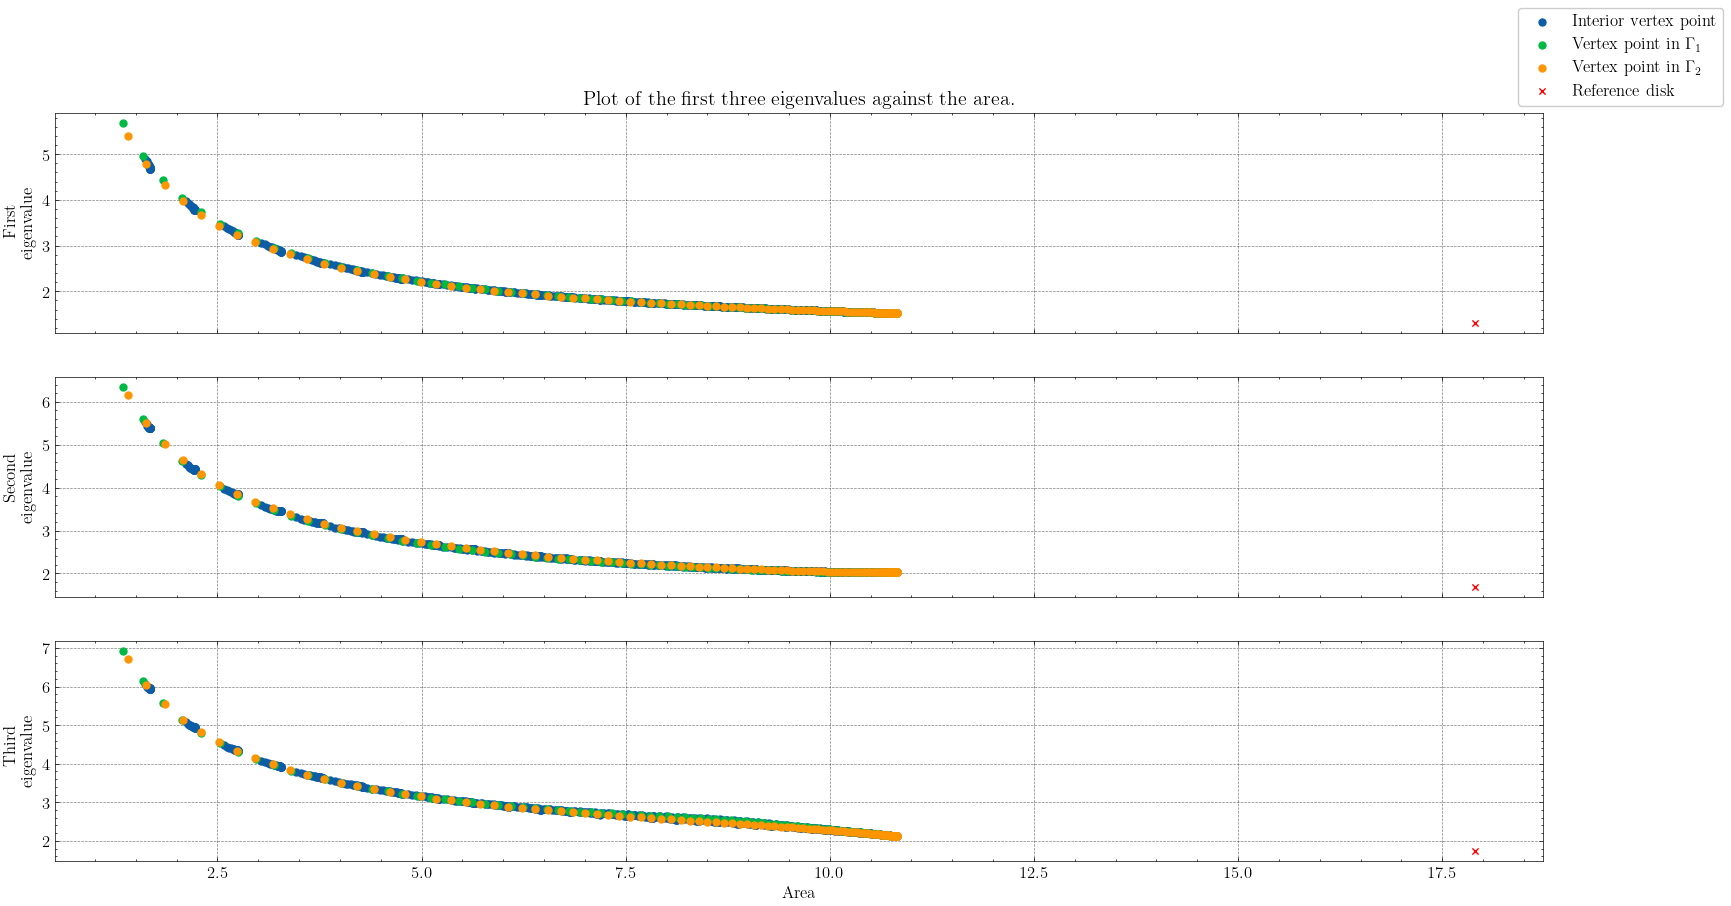
\includegraphics[width=\linewidth]{Images/Dirac/triangles/triangle_perimeter_first_eigenvalues.png}
    \captionof{figure}{Plot of the first three eigenvalues against the area with perimeter \(L = 15\) for triangular domains.}
    \label{dirac_triangle_model_perimeter}
\end{figure}

While for quadrilaterals (and for smooth domains in the next subsection) only random domains could be considered, for the problem among triangles, one can consider \textit{every} type of triangle by varying \((x,y)\) in \(\overline{R}\). Since the eigenvalues are continuous with respect to domain perturbations (in the next subsection, we will briefly formalize this concept using equation \eqref{dirac_perturbation_chapter_5}), it means that it is very unlikely that the conjectures studied for triangles (at least for \(m=1\)) do not hold, otherwise some jump would probably be found, for example in Figure \ref{dirac_triangle_3d_lambda1}. 

To finish this subsection, numerical evidence for Conjecture \ref{polya_szego_conjecture_dirac} for \(m=1\) is presented in Figures \ref{dirac_polya_szego_evidence_pentagons}, \ref{dirac_polya_szego_evidence_hexagons}, \ref{dirac_polya_szego_evidence_heptagons} and \ref{dirac_polya_szego_evidence_octagons}. For the sake of brevity, we only present the results for the first eigenvalue, although similar results were found for the second and third eigenvalues. As it is possible to check, the \(n\)-sided polygon with the least first eigenvalue is the regular polygon, with \(n=5,6,7,8\).

\begin{figure}[!htb]
    \centering
    \begin{minipage}[b]{0.45\textwidth}
        \centering
        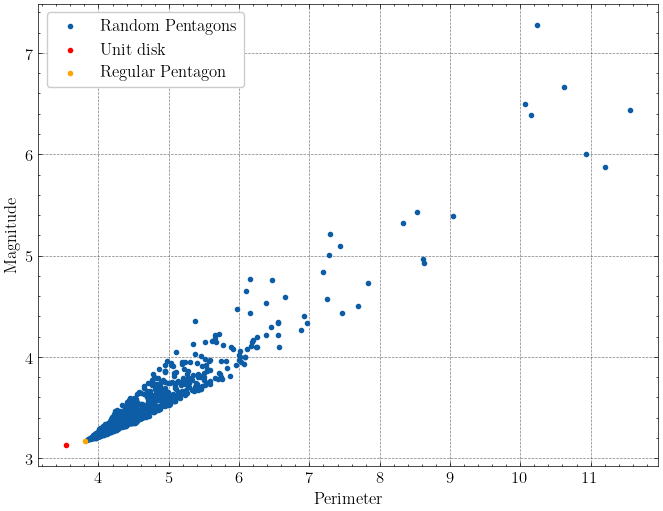
\includegraphics[width=\textwidth]{Images/Dirac/Polygons/pentagons.png}
    \caption{Numerical simulations in the first eigenvalue of general pentagons.}
    \label{dirac_polya_szego_evidence_pentagons}
    \end{minipage}
    \hfill
    \begin{minipage}[b]{0.45\textwidth}
        \centering
        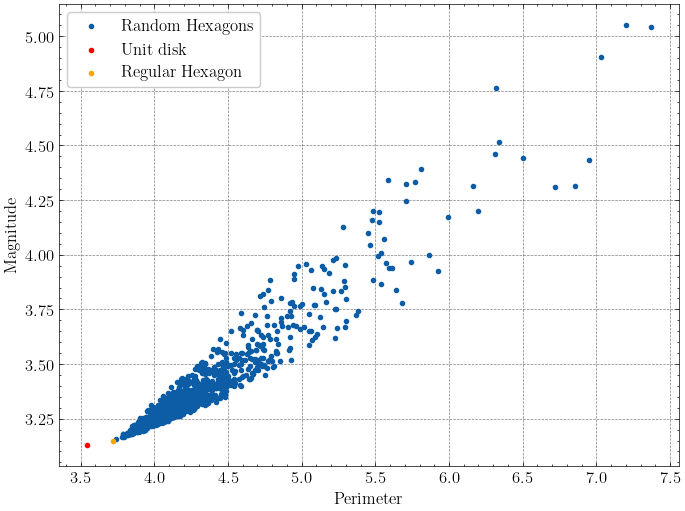
\includegraphics[width=\textwidth]{Images/Dirac/Polygons/hexagons.png}
    \caption{Numerical simulations in the first eigenvalue of general hexagons.}
    \label{dirac_polya_szego_evidence_hexagons}
    \end{minipage}

    \vspace{0.5cm}

    \begin{minipage}[b]{0.45\textwidth}
        \centering
        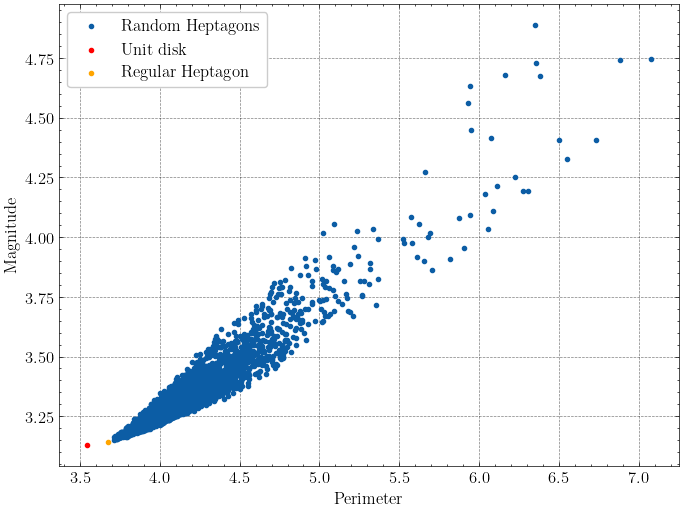
\includegraphics[width=\textwidth]{Images/Dirac/Polygons/heptagons.png}
    \caption{Numerical simulations in the first eigenvalue of general heptagons.}
    \label{dirac_polya_szego_evidence_heptagons}
    \end{minipage}
    \hfill
    \begin{minipage}[b]{0.45\textwidth}
        \centering
        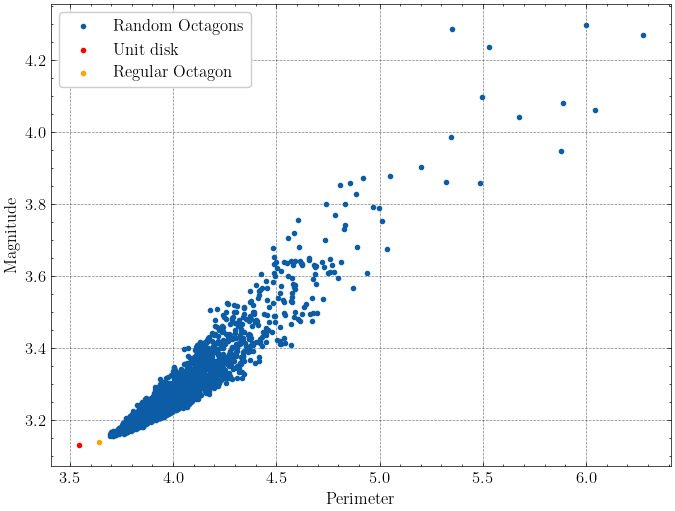
\includegraphics[width=\textwidth]{Images/Dirac/Polygons/octagons.png}
    \caption{Numerical simulations in the first eigenvalue of general octagons.}
    \label{dirac_polya_szego_evidence_octagons}
    \end{minipage}
\end{figure}

\subsection{Results in smooth domains}

In this last subsection, the behavior of the spectrum in smooth (connected) domains with unit area is studied. Here, we fix \(m=1\). The reason is twofold: first, the shape of the domains can be arbitrary and the numerical approximations are more reliable; second, one can also consider the domain which minimizes the third eigenvalue.

In order to generate random smooth domains, periodic B-spline interpolation (e.g. \cite{de1978practical} for details) for each component of a vector in \(\mathbb{R}^2\) was used. One starts by generating randomly five points (using a uniform distribution), fitting a periodic B-spline on this points for each component, drawing the two-dimensional B-spline, and checking for auto-intersections\footnote{Unfortunately, such sampling of smooth domains is not representative of the set of all smooth domains. For example, generating complex non-convex domains (like star-shape domains) may be impossible.}. If it does not auto-intersect, then it is a valid domain. Figure \ref{dirac_smooth_random_domain} presents an example.

\begin{figure}[!htb]
    \centering
    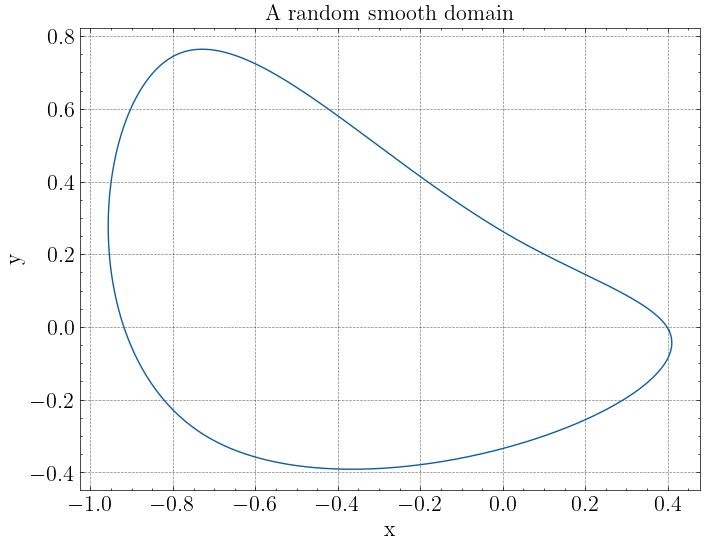
\includegraphics[width=0.55\linewidth]{Images/Dirac/smooth/random_smooth_domain.png}
    \captionof{figure}{Smooth domain generated by B-splines.}
    \label{dirac_smooth_random_domain}
\end{figure}

The results correspond to the ones presented in sections \ref{chap_numerics_dirac_quad_section} and \ref{chap_numerics_dirac_triangles_section}. In Figure \ref{dirac_smooth_domains_scatter_all_eigs} a scatter plot of the first three eigenvalues as a function of the perimeter is shown. Once again, analogously to the Laplacian, Conjecture \ref{conjecture_faber_krahn} appears to hold for the Dirac operator with infinite-mass boundary conditions. As seen in Figure \ref{dirac_first_three_eigenvalues_quad_m_1}, some ``outlier'' domains have a third eigenvalue that is smaller than the third eigenvalue on the disk, which suggests that the minimizers of the third Dirac and Laplace eigenvalues do not coincide.
Figures \ref{dirac_smooth_domains_scatter_benguria} and \ref{dirac_smooth_domains_scatter_benguria_third} are related to the ratio of the first eigenvalues and the spectral gap between them. Something analogous to the Ashbaugh-Benguria Theorem for the Laplacian also seems to hold for the Dirac operator.

\begin{figure}[!htb]
    \centering
    \begin{minipage}[c]{0.8\textwidth}
        \centering
        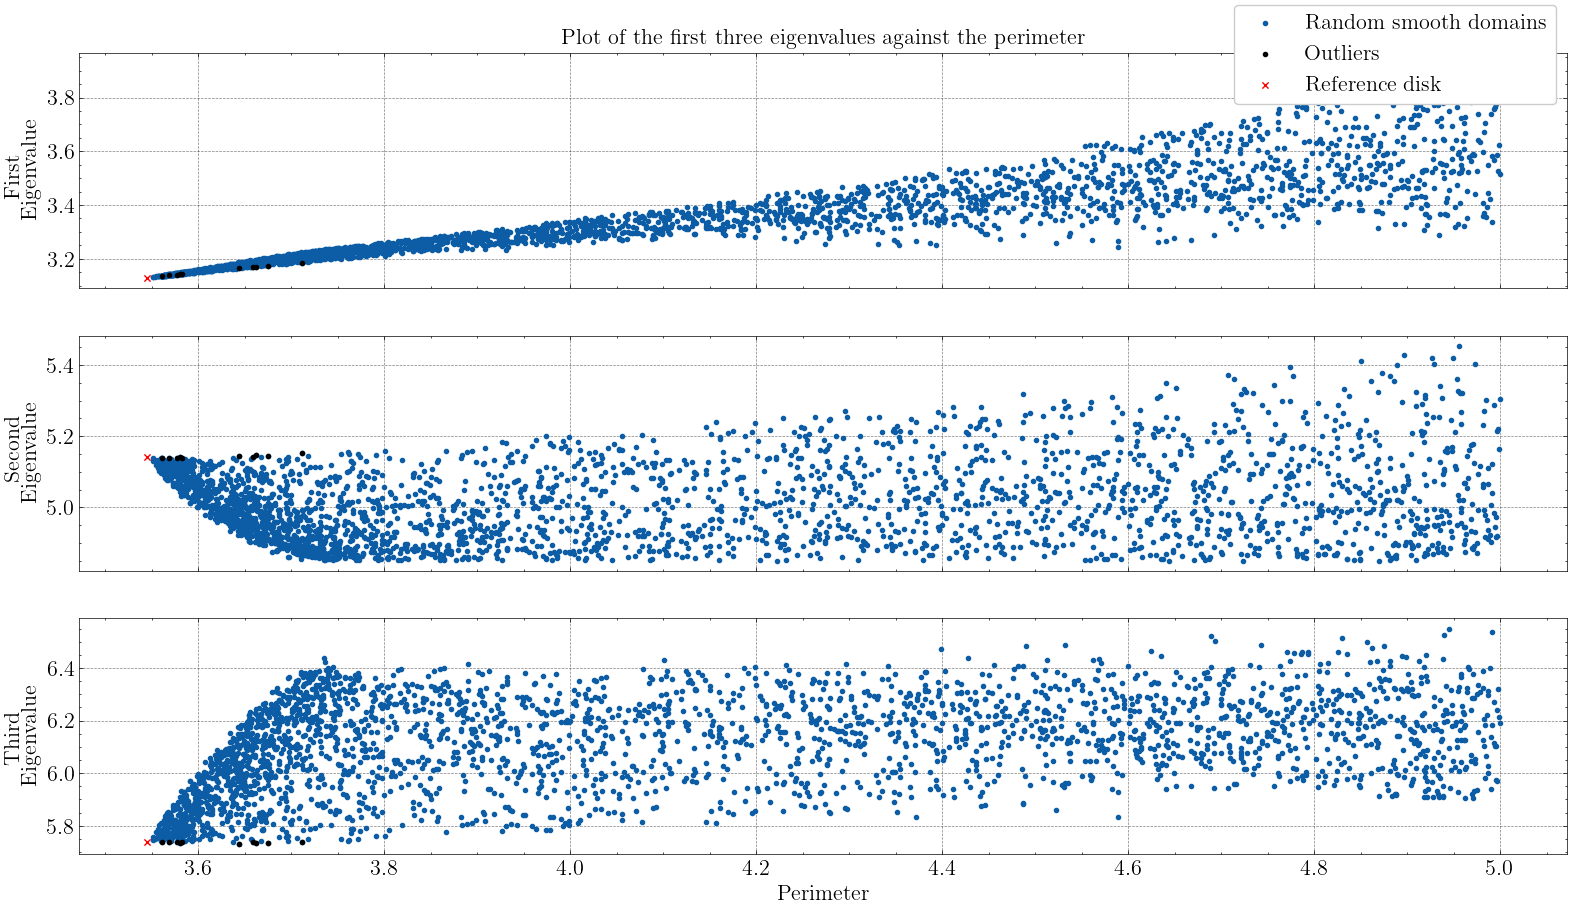
\includegraphics[width=\textwidth]{Images/Dirac/smooth/smooth_domains_scatter_all_eigs_.png}
        \caption{Magnitude of the first three eigenvalues plotted against the perimeter length in smooth domains. The ``outliers'' marked in black represent the domains in which the third eigenvalue is less than the third eigenvalue of the disk.}
        \label{dirac_smooth_domains_scatter_all_eigs}
    \end{minipage}

    \vspace{0.5cm}

    \begin{minipage}[c]{0.45\textwidth}
        \centering
        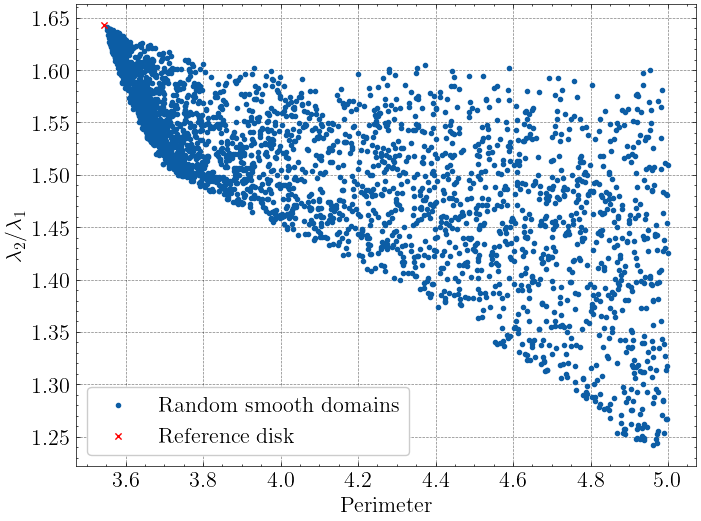
\includegraphics[width=\textwidth]{Images/Dirac/smooth/smooth_domains_scatter_benguria.png}
        \caption{Ratio between the first two eigenvalues \(\frac{\lambda_2}{\lambda_1}\) for smooth domains.}
        \label{dirac_smooth_domains_scatter_benguria}
    \end{minipage}
    \hfill
    % \begin{minipage}[c]{0.32\textwidth}
    %     \centering
    %     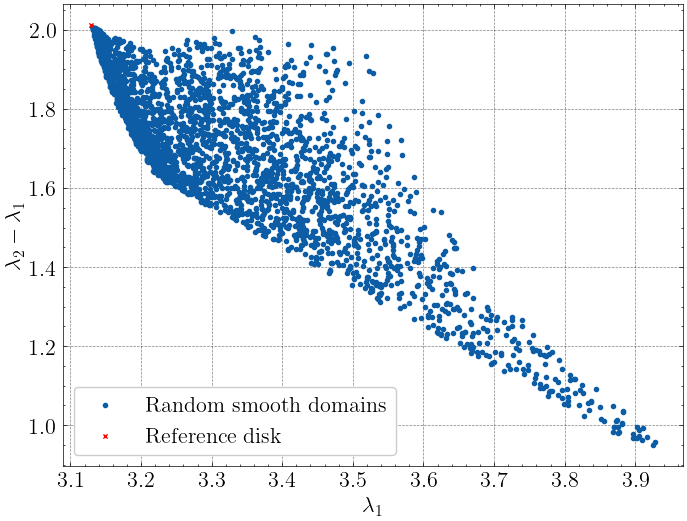
\includegraphics[width=\textwidth]{Images/Dirac/smooth/smooth_domains_scatter_gap.png}
    %     \caption{Spectral gap \(\lambda_2-\lambda_1\).}
    %     \label{dirac_smooth_domains_scatter_gap}
    % \end{minipage}
    % \hfill
    \begin{minipage}[c]{0.45\textwidth}
        \centering
        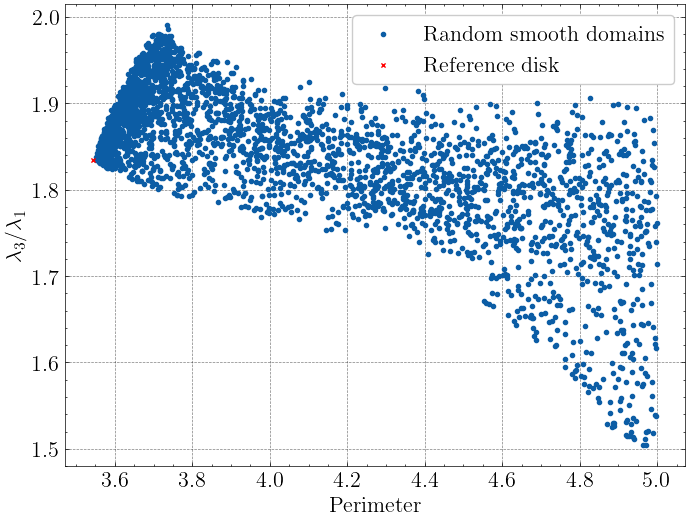
\includegraphics[width=\textwidth]{Images/Dirac/smooth/smooth_domains_scatter_benguria_third.png}
        \caption{Ratio between the third and first eigenvalues \(\frac{\lambda_3}{\lambda_1}\) for smooth domains.}
        \label{dirac_smooth_domains_scatter_benguria_third}
    \end{minipage}
\end{figure}

Next, we search for the domain with the smallest third eigenvalue, and thus look for the minimizer of the functional
\begin{equation*}%\label{dirac_min_third_func}
    \mathcal{F}(\Omega) = \lambda_3(\Omega).
\end{equation*}

In general, one can address minimization problems in Banach spaces using the notion of \textit{Fréchet}-derivative. In shape optimization problems, for the eigenvalues of an elliptic operator, one can use the variational formula for its eigenvalues. For example, the variational formula \eqref{append_variational_form_laplacian} proved in Theorem \ref{spec_lap_pre} can be used to derive some results for the Laplace-Dirichlet problem. In fact, let \(\Omega_t = \varphi(t)(\Omega)\) be a small perturbation of \(\Omega\) in the parameter \(t\), where \(\varphi(t)\) is a diffeomorphism for small values of \(t\) defined by
\begin{equation}\label{dirac_perturbation_chapter_5}
    \varphi(t) = I + t W,
\end{equation}
for some fixed vector field \(W\) and \(\Omega_0 = \Omega\). Let  \(\lambda_k(t)\) be an eigenvalue of the Laplace operator with Dirichlet boundary conditions on the domain \(\Omega_t\) and \(u^{(k)}_t\) its \(L^2\) normalized eigenfunction in \(H^1_0(\Omega_t)\). If \(\lambda_k\) has multiplicity one (if it is simple) and \(\Omega\) is of class \(C^2\) or convex, then
\begin{equation}\label{hadamard_dirac_numerics_chap}
    \lambda'_k(0) =- \int_{\partial\Omega} \left(\frac{\partial u^{(k)}_0}{\partial n}\right)^2 V\cdot n d \sigma.
\end{equation}
For more details, we refer to \cite{henrot2006extremum} and \cite{kato2013perturbation}. Numerically, equation \eqref{hadamard_dirac_numerics_chap} can then be used in shape optimization problems for the Dirichlet Laplacian \ac{BVP}, for example in gradient-based methods like gradient descent.
As of the moment of writing, the author is not aware of any such closed form for the derivative of the eigenvalues of the Dirac operator. Therefore, two different strategies were considered to solve the unconstrained minimization problem
\begin{equation}\label{dirac_unconstrained_min_lambda_3}
    \min_{\substack{\Omega \subset \mathbb{R}^2 \\ \abs{\Omega}=1}} \mathcal{F}(\Omega).
\end{equation}

Starting with a given domain \(\Omega\), \(\mathcal{F}\) can be minimized using the \ac{BFGS} algorithm, e.g. see \cite{andrei2022modern}, a quasi-Newton method that uses the local curvature of \(\mathcal{F}\) to find the descent direction given by an approximation of the Hessian matrix. As in most optimization techniques, we need, however, to compute the derivative of the objective function, since we are solving the equation \(\mathcal{F}' =0\). In our case, this can only be done numerically using, for example, finite differences. The second method is the multidimensional Nelder-Mead direct search method, which we also refer to \cite{andrei2022modern}. As in the bracketing algorithm used in finding the singularities on the graph of the smallest singular value, the Nelder-Mead method does not need any information on the derivative and relies solely on evaluations of the objective function \(\mathcal{F}\) to bracket the local minima, which we approximate using a heuristic strategy with a multidimensional simplex is used to approximate it.

To apply both the \ac{BFGS} and the Nelder-Mead algorithms, one starts by parameterize the domain \(\Omega_0\) with the lowest third eigenvalue by a polar parameterization. This is achieved by considering a sample of \(N\) boundary points from the domain, considering its polar coordinates, and finding the coefficients of the trigonometric interpolation. More precisely, let \(M\) be the order of the trigonometric interpolation. Assume that the radial part of each boundary point of \(\Omega_0\) can be parametrized by \(r(\theta)\), where \(\theta \in (0, 2\pi)\). In that case, one uses the approximation
\[
    r(\theta_i) \approx a_0 + \sum_{m=1}^{M}a_m \cos(m \theta_i) + \sum_{m=1}^{M}b_m \sin(m \theta_i),
\]
where \(\theta_i\) is the polar part of the sample point \(i\) with \(i=1,\dots,N\). Then, the system
\[
    \begin{bmatrix}
        1 & \cos(1 \theta_1) & \cos(2 \theta_1) & \dots & \cos(M \theta_1) & \sin(1 \theta_1) & \dots & \sin(M \theta_1)\\
        \vdots & \vdots & \vdots & \vdots & \vdots & \vdots & \vdots & \vdots\\
        1 & \cos(1 \theta_N) & \cos(2 \theta_N) & \dots & \cos(M \theta_N) & \sin(1 \theta_N) & \dots & \sin(M \theta_N)
    \end{bmatrix}_{N\times(2M+1)}
    \begin{bmatrix}
        a_0\\
        \vdots\\
        b_M
    \end{bmatrix}
    =
    \begin{bmatrix}
        r(\theta_1)\\
        \vdots\\
        r(\theta_N)\\
    \end{bmatrix}
\]
can be solved by least squares. Notice that problem \eqref{dirac_unconstrained_min_lambda_3} is now a finite-dimensional problem since every domain is a vector of coefficients in \(\mathbb{R}^{2M+1}\). Of course, one must still scale the generated domain so that it has a unit area.

Figure \ref{dirac_nelder_mead_domain} presents an (almost) optimal domain \(\Omega^\star\) which minimizes the third eigenvalue of the Dirac operator with infinite-mass boundary conditions. This shape was obtained through the Nelder-Mead algorithm. The third eigenvalue of the problem in this domain is approximately \(\lambda_3 \approx 5.63787728\) and the perimeter length of \(\Omega^\star\) is \(L \approx 5.2650031\). In Figure \ref{dirac_val_third} we validate our findings by plotting the (continuous) family of one-parameter transformations (known as the Minkowski sum) from the unit disk \(\mathbb{D}\) to \(\Omega^\star\), given by
\[
   \Omega_t = (1-t)\mathbb{D} + t \Omega^\star, \; 0 \leq t \leq 1.
\]
\begin{figure}[!htb]
    \centering
    \begin{minipage}{.5\textwidth}
        \centering
        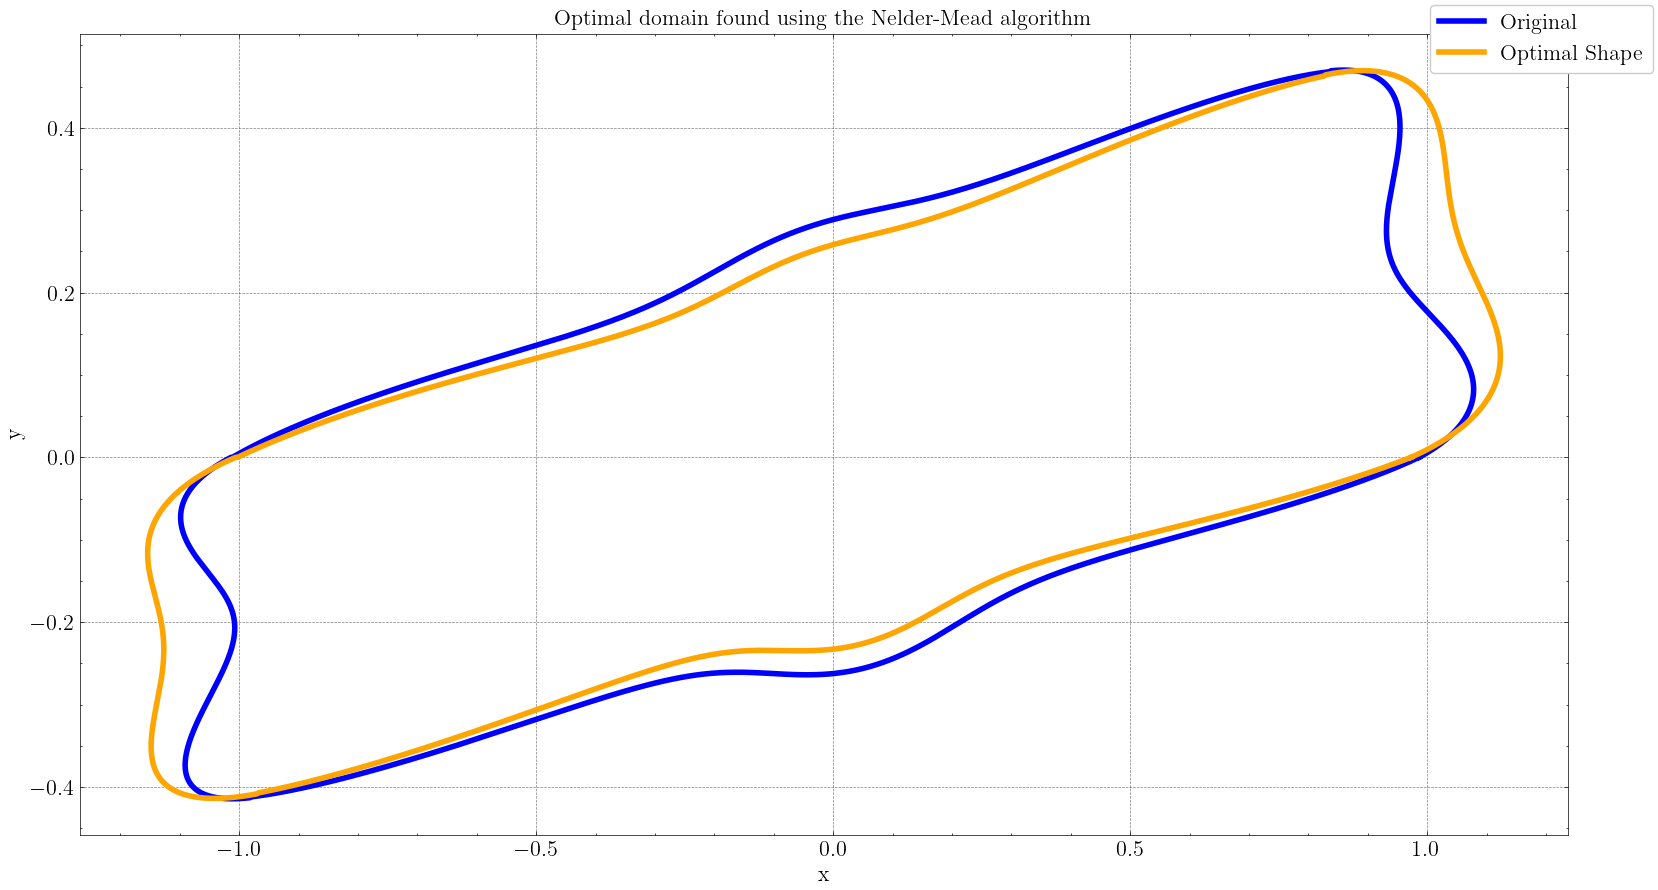
\includegraphics[width=0.9\linewidth]{Images/Dirac/smooth/nelder_mead_optimal.png}
        \captionsetup{width=0.8\linewidth} % Adjust the width of the caption
        \captionof{figure}{Optimal domain \(\Omega^\star\) (drawn in orange) and the initial domain (in blue) used in the first iteration of the Nelder-Mead algorithm.}
        \label{dirac_nelder_mead_domain}
    \end{minipage}%
    \hfill
    %\hspace{0.5cm} % Add some horizontal space between the figures
    \begin{minipage}{.5\textwidth}
        \centering
        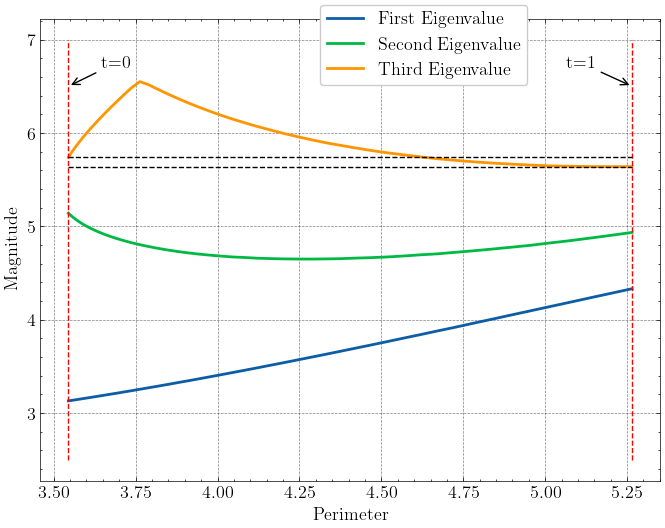
\includegraphics[width=0.8\linewidth]{Images/Dirac/smooth/dirac_val_third.png}
        \captionsetup{width=0.8\linewidth} % Adjust the width of the caption
        \captionof{figure}{The first three eigenvalues in domains defined by the Minkowski sum \(\Omega_t\) and plotted for the values of \(t\in [0,1]\) increasing from left to right.}
        \label{dirac_val_third}
    \end{minipage}
\end{figure}

As mentioned earlier, the \ac{BFGS} method was also employed. However, this method did not yield meaningful results. We attribute this to the proximity of the initial domain to the global minimizer, leading to a natural loss of precision when calculating the gradient through finite differences. The combination of these issues, along with the finite (albeit accurate due to the smoothness of the domains being considered) numerical precision of the \ac{MFS}, justifies the lack of convergence of the \ac{BFGS} method.

\begin{remark}
    One can not fail to point out a valid criticism to approach the minimization problem \eqref{dirac_unconstrained_min_lambda_3}: since we only parametrized the radial part of the domain's boundary, we always end up with star-like shapes. Moreover, in our case, the order of the trigonometric interpolation was low, with \(M=4\). We note however that, by increasing the order of interpolation, the dimension of the optimization space also increases, and already in \(\mathbb{R}^9\) it is very hard for a direct search method like Nelder-Mead to find a local minimum. The option to consider only the radial part, instead of both cartesian components, was also a way to reduce the dimensionality of the problem. 
\end{remark}

Finally, the normalized eigenfunction associated with the optimal third eigenvalue of domain \(\Omega^\star\) is shown in Figure \ref{dirac_optimal_plots_eigenfunctions}.

\begin{figure}[!htb]
    \centering
    \begin{minipage}[b]{0.45\textwidth}
        \centering
        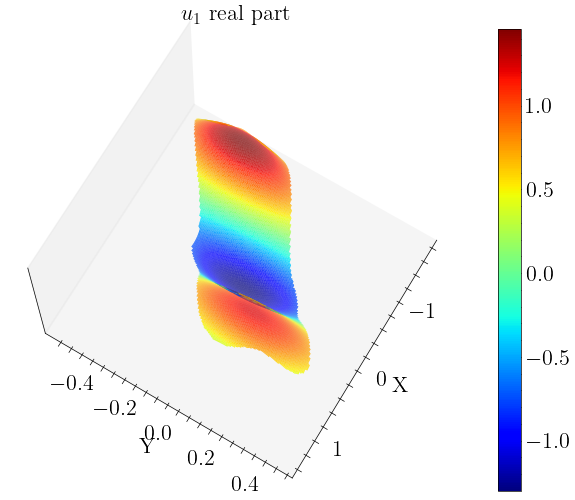
\includegraphics[width=0.75\textwidth]{Images/Dirac/smooth/optimal_lambda3_m_1_u1_re.png}
%\caption{Network 1}
    \end{minipage}
    \hfill
    \begin{minipage}[b]{0.45\textwidth}
        \centering
        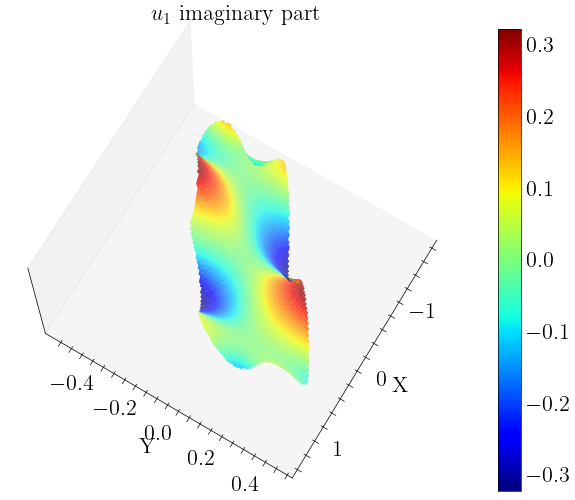
\includegraphics[width=0.75\textwidth]{Images/Dirac/smooth/optimal_lambda3_m_1_u1_im.png}
%\caption{Network 2}
    \end{minipage}

    \vspace{0.5cm}

    \begin{minipage}[b]{0.45\textwidth}
        \centering
        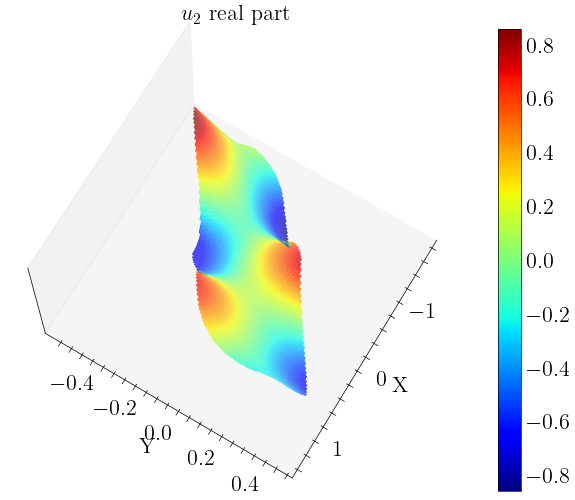
\includegraphics[width=0.75\textwidth]{Images/Dirac/smooth/optimal_lambda3_m_1_u2_re.png}
%\caption{Network 3}
    \end{minipage}
    \hfill
    \begin{minipage}[b]{0.45\textwidth}
        \centering
        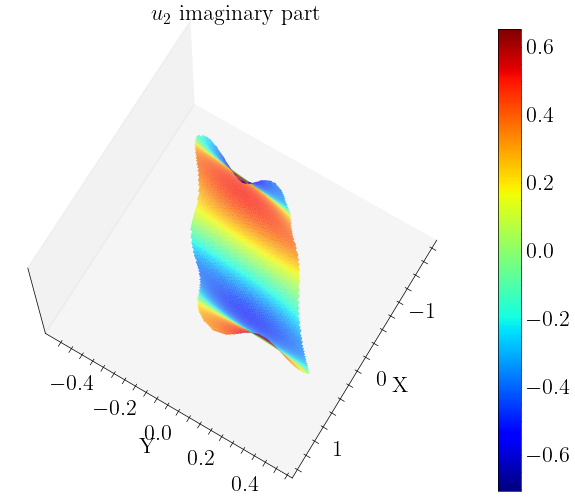
\includegraphics[width=0.75\textwidth]{Images/Dirac/smooth/optimal_lambda3_m_1_u2_im.png}
%\caption{Network 4}
    \end{minipage}
    \caption{Real and imaginary parts of \(u_1\) and \(u_2\) of the third eigenfunction \(\mathbf{u}=\begin{bmatrix} u_1\\ u_2 \end{bmatrix}\) associated with the optimal domain \(\Omega^\star\).}
    \label{dirac_optimal_plots_eigenfunctions}
\end{figure}

% \begin{figure}[!htb]
%     \centering
%     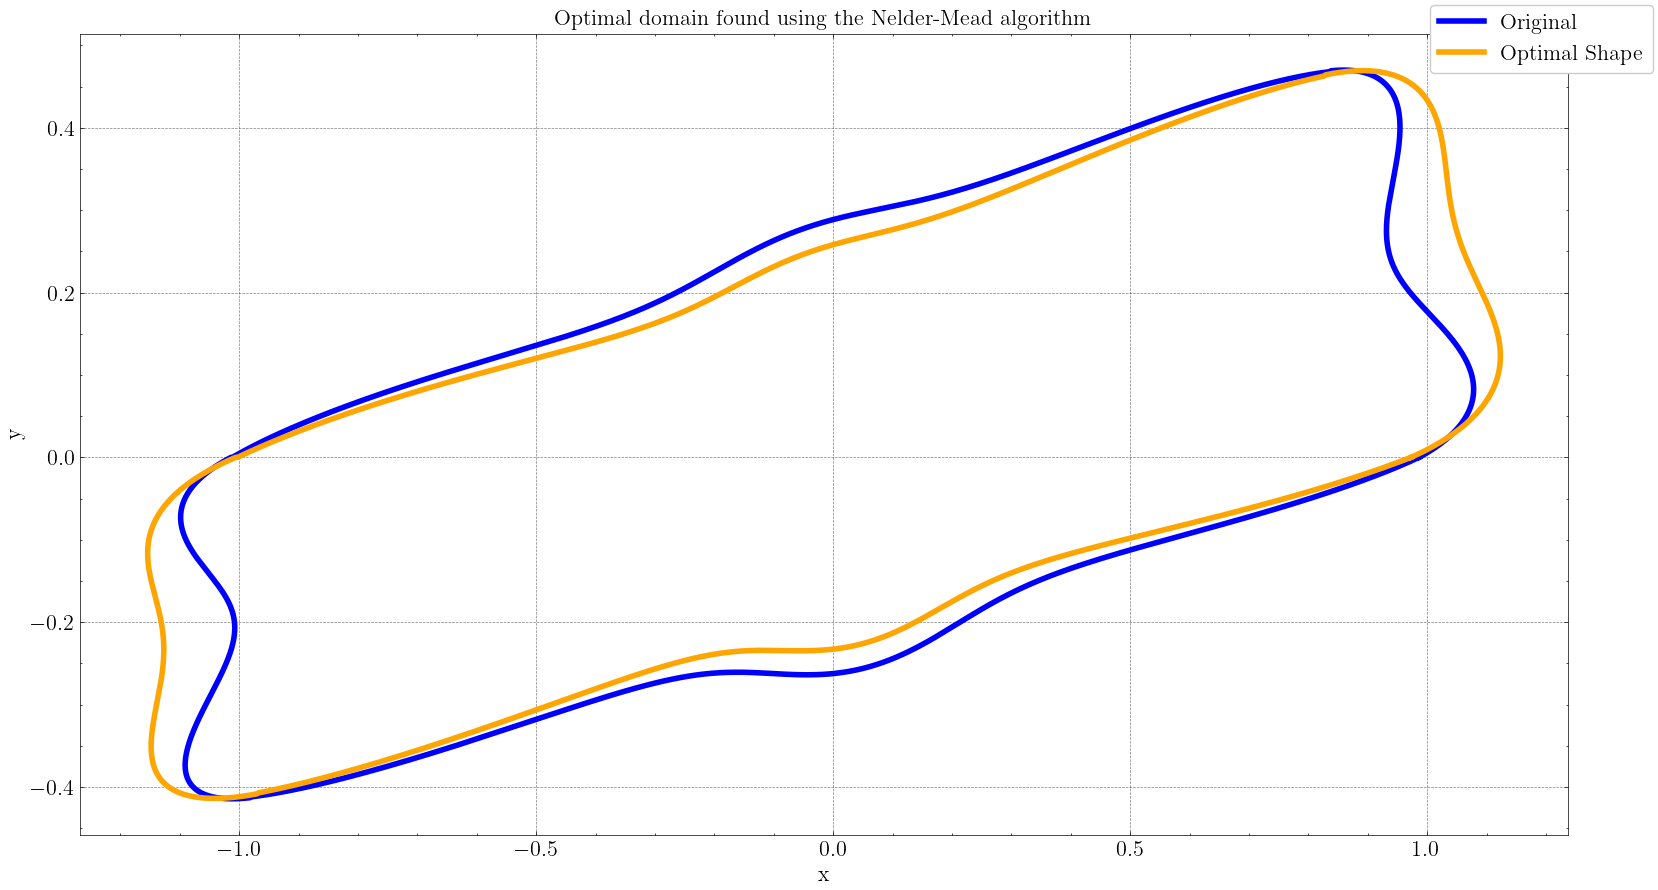
\includegraphics[width=0.75\linewidth]{Images/Dirac/smooth/nelder_mead_optimal.png}
%     \captionof{figure}{Some smooth domain generated by B-splines.}
%     \label{dirac_nelder_mead_domain}
% \end{figure}

% \begin{figure}[!htb]
%     \centering
%     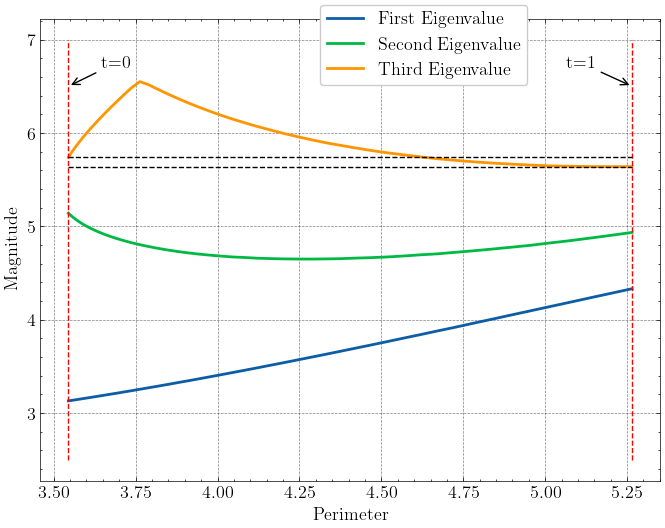
\includegraphics[width=0.75\linewidth]{Images/Dirac/smooth/dirac_val_third.png}
%     \captionof{figure}{Some smooth domain generated by B-splines.}
%     \label{dirac_val_third}
% \end{figure}

\section{Transmission problem}\label{numerical_transmission_simulations}

We now recall the set of equations introduced in the subsection \ref{domain_decomp_problem},
\begin{align}\label{transmission_num}
    \begin{cases}
    - \nabla k_i \left(\nabla u_i\right) = f_i, & \text{in }\Omega_i\\
    u_1 - u_2 = 0, & \text{on }\gamma\\
    k_1 \frac{\partial u_1}{\partial \mathbf{n_1}} + k_2 \frac{\partial u_2}{\partial  \mathbf{n_2}} = 0, & \text{on }\gamma\\
    u_i = 0, & \text{on }\Gamma_i,
    \end{cases}
\end{align}
for \(i=1, 2\).

Problem \ref{transmission_num} can be understood as a domain decomposition problem, where \(\Omega \subset \mathbb{R}^2\) is divided into two non-overlapping regions \(\Omega_1\) and \(\Omega_2\) such that \(\overline{\Omega} = \overline{\Omega_1} \cup \overline{\Omega_2}\). The interface between \(\Omega_1\) and \(\Omega_2\) is denoted by \(\gamma = \partial\Omega_1 \cap \partial\Omega_2\) and the rest of the boundary of each domain by \(\Gamma_i = \partial\Omega_i\setminus{\gamma}, \, i=1, 2\). In what follows, the source functions \(f_i\) at each domain are taken to be constant\footnote{Like in article \cite{gustafsson2019error}, in this work we only considered \(f_i=1\). In any case, we will still have a jump in the material parameter \(k\), if \(k_1 \neq k_2\).
%Working with different \textit{continuous} source functions should make no difference in the result if a closed-form non-homogeneous solution exists (to be explained in the next pages, where we will also present how to deal with general and continuous source functions).
}. Recall that \(k_1 \geq k_2 > 0\) are constants and \(\mathbf{n_i}\) is the (normalized) outward normal to \(\Omega_i, i=1, 2\), where we write \(\mathbf{n}= \mathbf{n_1}=- \mathbf{n_2}\) when \(\mathbf{n}\) is restricted to the interface.

The procedure presented here is based on \cite{alves2005new} and \cite{alves2021domain}. Given that \(f_i = 1, \, i=1, 2\), a solution of \eqref{transmission_num} can be found by taking the following steps:
\begin{enumerate}
    \item \label{chapter_numerics_t_p_particular_prodecure} Find a non-homogeneous solution (recall footnote \ref{particular_solutions_footnote} in Chapter \ref{chap:numerical}) for the non-homogeneous problem
    \[
        \begin{cases}
            -\Delta u_1^{NH} = \frac{1}{k_1}\\
            -\Delta u_2^{NH} = \frac{1}{k_2},
        \end{cases}
    \]
    in \(\mathbb{R}^2\) which does not necessarily satisfy the boundary and interface conditions in \eqref{transmission_num}. This can easily be done, and
    \[
        \begin{cases}
            u_1^{NH} = -\frac{x_1^2 + x_2^2}{4k_1}\\
            u_2^{NH} = -\frac{x_1^2 + x_2^2}{4k_2}
        \end{cases}
    \]
    are some possible non-homogeneous solutions;
    \item Then we solve the homogeneous problem 
    \begin{align}\label{transmission_num_homo}
        \begin{cases}
        - \Delta u_i^H = 0, & \text{in }\Omega_i\\
        u_1^H - u_2^H = u_2^{NH}- u_1^{NH}, & \text{on }\gamma\\
        k_1 \frac{\partial u_1^H}{\partial \mathbf{n_1}} - k_2 \frac{\partial u_2^H}{\partial  \mathbf{n_1}} = k_2 \frac{\partial u_2^{NH}}{\partial  \mathbf{n_1}}  - k_1 \frac{\partial u_1^{NH}}{\partial  \mathbf{n_1}}, & \text{on }\gamma\\
        u_i^H = - u_i^{NH}, & \text{on }\Gamma_i,
        \end{cases}
    \end{align}
    for \(u_1^H\) and \(u_2^H\);
    \item Finally, the solution of \eqref{transmission_num} is \(u_i = u_i^H + u_i^{NH}\).
\end{enumerate}
\begin{remark}
    For general (possibly different) source functions, the steps above can also be used: however, it may not be possible to find a closed form solution in the first step. In this case, the problem in step \ref{chapter_numerics_t_p_particular_prodecure} must be solved numerically. A popular choice is to use \acp{RBF}, e.g. \cite{golberg1996improved}, for example the thin plate spline
    \[
        \varphi(r) = r^2 \log r,     
    \]
    and, for each subdomain \(\Omega_i\) with \(i=1,2\) find the coefficients \(\alpha_j^{(i)}\) in \(f_i(x_k^{(i)}) =\tilde{f}_i(x_k^{(i)}) = \sum_{j=1}^{n} \alpha_j^{(i)} \varphi_j(x_k^{(i)})\) using least square methods, where \(\tilde{f}_i\) is an approximation for the source function \(f_i\) given by linear combinations of thin plate splines, \(x_k^{(i)}\) are collocation points for \(k=1,\dots,M^{(i)}\), \(\varphi_j(r) = \varphi(\abs{x^{(i)}-y_j})\) and \(y_j \in \mathbb{R}^2, \, j =1,\dots, N\), is the \ac{RBF} center, which is analogous to the concept of \textit{source points} in the \ac{MFS}. Finally, one can analytically solve for the \(\Psi_j\) functions in the polar Poisson equation \(\frac{1}{r}\left(r \frac{\partial}{\partial r}\Psi_j\right)  = \varphi_j\) with \(j=1,\dots,N\) in \(\mathbb{R}^2\), to recover the approximate non-homogeneous solutions \(u_1^{NH}\) and \(u_2^{NH}\), given by
    \begin{align*}
        u_i^{NH}(x) = \sum_{j=1}^{N} \alpha_j^{(i)} \Psi_j(x-y_j^{(i)}).
    \end{align*}
    In \cite{alves2005new} and \cite{alves2021domain} a different approach was suggested using the fundamental solutions of the Helmholtz equation instead of the classical \acp{RBF}; that method is known today as \textit{Kansa-MFS method}.
\end{remark}

In what follows, the numerical results illustrate the accuracy of the method in simply connected 2D domains. Let \(N^{(i)}\) denote the number of source points at each domain and \(N=N^{(1)}+N^{(2)}\). We denote the approximate solution by
\[
    \tilde{u} = \begin{cases}
        \tilde{u}_1, & \text{in } \Omega_1\\
        \tilde{u}_2, & \text{in } \Omega_2,
    \end{cases}
\]
where
\begin{align*}
    &\tilde{u}_1(x) = \sum_{j=1}^{N^{(1)}} \alpha^{(1)}_j \Phi\left(x-y_j^{(1)}\right)\\
    &\tilde{u}_2(x) = \sum_{j=1}^{N^{(2)}} \alpha^{(2)}_j \Phi\left(x-y_j^{(1)}\right).
\end{align*}
Let \(M^{(i)}\) be the number of boundary collocation points \(x^{(i)}_{m}\) for each \(\Omega_i\) and \(M=M^{(1)}+M^{(2)}\). We also consider \(Q\) interface points \(z_q \in \gamma\) with \(q=1,\dots,Q\). Then, the full block system is written as
\begin{equation}\label{MFS_transmission_classical_matrices_system}
    \renewcommand{\arraystretch}{1.75} % Increase spacing between rows of the matrices
    {\underbrace{\begin{bmatrix}
        \left[\Phi\left(x^{(1)}_{m}-y_j^{(1)}\right)\right]_{M^{(1)}\times N^{(1)}} & [0]_{M^{(1)}\times N^{(2)}} \\
        [0]_{M^{(2)}\times N^{(1)}} & \left[\Phi\left(x^{(2)}_{m}-y_j^{(2)}\right)\right]_{M^{(2)}\times N^{(2)}} \\
        \left[\Phi\left(z_q-y_j^{(1)}\right)\right]_{Q\times N^{(1)}} & \left[-\Phi\left(z_q-y_j^{(2)}\right)\right]_{Q\times N^{(2)}} \\
        \left[k_1\partial_n \Phi\left(z_q-y_j^{(1)}\right)\right]_{Q\times N^{(1)}} & \left[-k_2 \partial_n \Phi\left(z_q-y_j^{(2)}\right)\right]_{Q\times N^{(2)}}
    \end{bmatrix}}_A}
    {\underbrace{\begin{bmatrix}
        \left[\alpha^{(1)}_j\right]\\
        \left[\alpha^{(2)}_j\right]
    \end{bmatrix}}_\alpha}=
    {\underbrace{\begin{bmatrix}
        \left[-u_1^{NH}(x^{(1)}_{m})\right]_{M^{(1)}\times 1}\\
        \left[-u_2^{NH}(x^{(2)}_{m})\right]_{M^{(2)}\times 1}\\
        \left[u_2^{NH}(z_q)-u_1^{NH}(z_q)\right]_{Q\times 1}\\
        \left[k_2 \partial_n u_2^{NH}(z_q)- k_1 \partial_n u_1^{NH}(z_q)\right]_{Q\times 1}\\
    \end{bmatrix}}_b}
\end{equation}
where the dimensions of the matrix \(A\) are \((M^{(1)}+M^{(2)}+2Q)\times(N^{(1)}+N^{(2)})\).

Most of the examples below do not have an analytical solution: only in the section \ref{transmission_val_subsection}, when we test the results against a known solution, we can compute the actual error everywhere. In the other cases, we only check for consistency errors which measure how accurately the interface and boundary conditions are satisfied:
\begin{itemize}
    \item \(\norm*{\tilde{u}_i - 0}_{L^2(\Gamma_i)}\), \(i=1, 2\): boundary collocation error;
    \item \(e_\gamma^0 = \norm*{\tilde{u}_1 - \tilde{u}_2}_{L^2(\gamma)}\), \(i=1, 2\): \(L^2\) error of \(\tilde{u}\) across \(\gamma\);
    \item \(e_\gamma^1 = \norm*{k_1 \partial_n\tilde{u}_1 - k_2 \partial_n\tilde{u}_2}_{L^2(\gamma)}\), \(i=1, 2\): \(L^2\) error of \(\partial_n\tilde{u}\) across \(\gamma\).
\end{itemize}
From a numerical point of view, let \(\mathcal{I}\) be the sample of test points. The \(L^2\) norm is discretized into the \ac{RMSE}\ which is equivalent to the \(l^2\) norm and is given by
\[
    \norm*{u-\tilde{u}}= \sqrt{\frac{1}{\#\mathcal{I}} \sum_{z \in \mathcal{I}} \abs{u(z)-\tilde{u}(z)}^2}.
\]
For every result below the number of sample test points is 5 times larger than the sample used to find the coefficients of the \ac{MFS}, and we fix \(k_2=1\) since the ratio \(\frac{k_1}{k_2}\) is responsible for the behavior of the solutions near the interface. 

\subsection{Numerical validation of the method}\label{transmission_val_subsection}

First, we start by testing the numerical algorithm for the unit disk \(\mathbb{D}\), with \(k_1=k_2=1\). From Theorem \ref{equivalence_transmission}, we know that the system of differential equations \eqref{transmission_num} is equivalent to the Poisson equation
\begin{align}\label{transmission_disk}
    \begin{split}
        -\Delta u = 1, & \text{ in } \mathbb{D}\\
        u = 0, & \text{ on } \partial\mathbb{D},
    \end{split}
\end{align}
and is easy to see that the exact solution of Equation \eqref{transmission_disk} is given in polar coordinates by \(u(r, \theta) = \frac{1-r^2}{4}\). 

\begin{figure}[!htb]
    \centering
    \begin{minipage}{.5\textwidth}
      \centering
      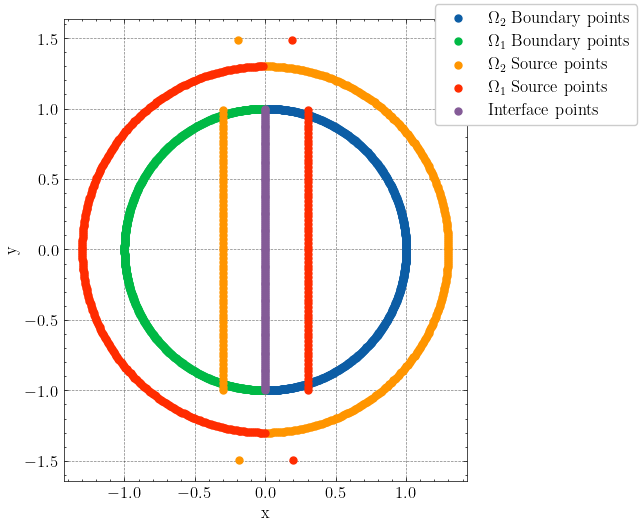
\includegraphics[width=0.9\linewidth]{Images/Transmission/Circle_val_col_points_600_150.png}
      \captionsetup{width=0.9\linewidth} % Adjust the width of the caption
      \captionof{figure}{Configuration of the boundary, source, and interface points. Each domain has 600 boundary points, 377 source points and the common interface has 100 points.}
      \label{transmission_disk_col}
    \end{minipage}%
    %\hspace{0.5cm} % Add some horizontal space between the figures
    \begin{minipage}{.5\textwidth}
      \centering
      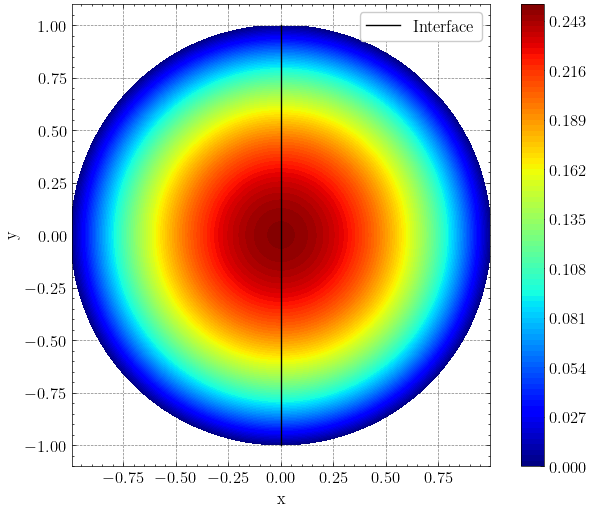
\includegraphics[width=0.8\linewidth]{Images/Transmission/Circle_val_contour_600_150.png}
      \captionsetup{width=0.9\linewidth} % Adjust the width of the caption
      \captionof{figure}{Numerical approximation of the solution \(u\) of the \ac{BVP} \eqref{transmission_disk} using the configuration presented in Figure \ref{transmission_disk_col}. The colorbar shows the values of \(u\).}
      \label{transmission_disk_plot}
    \end{minipage}
\end{figure}

The absolute error between the approximate solution and the exact solution can then be calculated for each domain point. The sample points to compute the absolute error were generated in a uniform grid and were also used to plot Figure \ref{transmission_disk_plot}. The method described at the end of the subchapter \ref{density_proofs_section}, below Remark \ref{density_remark_general_bc_and_hilbert}, was used to place the source points, where the coefficient \(\eta\) that controls the distance between the boundary \(\Gamma\) and the artificial boundary \(\hat{\Gamma}\) is \(0.3\).

\begin{table}[htbp]
    \centering
    \begin{tabular}{cccccc}
        \toprule
        \multirow{2}{*}{\textbf{Boundary/Interface Points}} & \multicolumn{2}{c}{\textbf{Boundary Error}} & \multicolumn{2}{c}{\textbf{Total Error}} \\
        \cmidrule(lr){2-3} \cmidrule(lr){4-5}
        & \textbf{Domain 1} & \textbf{Domain 2} & \textbf{Domain 1} & \textbf{Domain 2} \\
        \midrule
        600/150 & $9.759\times10^{-12}$ & $9.541\times10^{-12}$ & $1.465\times10^{-11}$ & $1.439\times10^{-11}$ \\
        500/100 & $3.667\times10^{-11}$ & $3.945\times10^{-11}$ & $9.382\times10^{-11}$ & $9.310\times10^{-11}$ \\
        412/100 & $3.721\times10^{-11}$ & $5.036\times10^{-11}$ & $9.652\times10^{-11}$ & $9.584\times10^{-11}$ \\
        \bottomrule
    \end{tabular}
    \caption{Numerical errors at the boundaries \(\partial\Omega_1\) and \(\partial \Omega_2\) and in the domains \(\Omega_1\) and \(\Omega_2\)}.
    \label{tab:transmission_results_1}
\end{table}


\begin{table}[htbp]
    \centering
    \begin{tabular}{cccc}
      \toprule
      \textbf{Boundary/Interface Points} & \textbf{Interface \(e_\gamma^0\) Error} & \textbf{Interface \(e_\gamma^1\) Error} & \textbf{Condition number} \\
      \midrule
      600/150 & $6.945\times10^{-11}$ & $1.841\times10^{-11}$ & $2.528\times 10^{19}$\\
      500/100 & $3.910\times10^{-10}$ & $1.100\times10^{-10}$ & $2.382\times 10^{18}$\\
      412/100 & $4.035\times10^{-10}$ & $1.342\times10^{-10}$ & $7.597\times 10^{17}$\\
      \bottomrule
    \end{tabular}
    \caption{Numerical errors at the interface \(\gamma\). The condition number of the matrix is also presented.}
    \label{tab:transmission_results_2}
\end{table}

The numerical results presented in Tables \ref{tab:transmission_results_1} and \ref{tab:transmission_results_2} are not yet optimal. When considering a larger value of \(\eta\), the results increase by more than two orders of magnitude, but this also leads to a significant increase in the already very high condition number of matrix \(A\) in the system \eqref{MFS_transmission_classical_matrices_system} (see Table \ref{tab:transmission_results_2}), as expected. Despite this, the results show great promise, which was anticipated due to the domain's smoothness.

As mentioned previously, the \ac{MFS} yields better results in highly regular domains, even when considering curved geometries. However, increasing the number of boundary and interface collocation points improves the accuracy of the solution. It is important to note that a larger number of points also makes the condition number grow, making solving the problem accurately more challenging.

% The inclusion of ``corner'' source points, as depicted in Figure \ref{transmission_disk_col}, also significantly impacts the method's accuracy. These source points were strategically added to capture the behavior near the interface corner. Notice that the source points for one of the domains can be inside the other domain as the solution will be split into two parts.

\subsection{Results for the rectangle}

In this subchapter, we focus on a rectangular domain \([-1, -0.5] \times [1, 0.5]\) with a vertical interface along the line \(x=0\). We aim to study the problem for \(k_1 \neq k_2\), where \(k_2=1\) is fixed. The results presented in Table \ref{tab:transmission_results_rectangle} for each value of \(k\) were obtained using 600 boundary points and 404 source points in each domain, with 150 interface points and \(\eta=0.08\).

\begin{figure}[!htb]
    \centering
    \begin{minipage}{.5\textwidth}
      \centering
      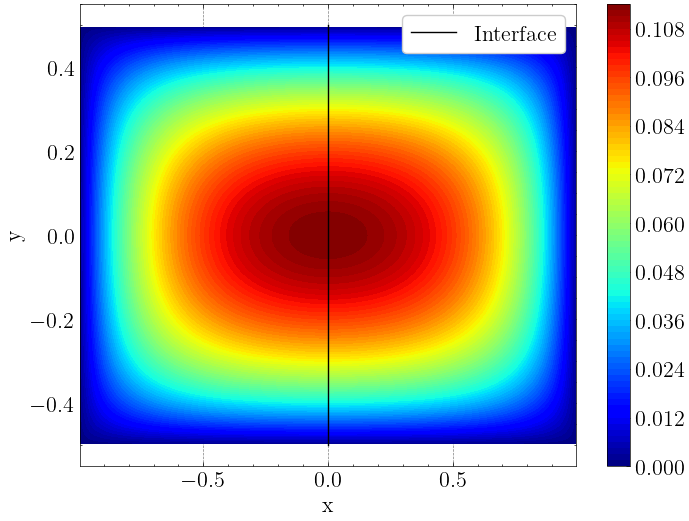
\includegraphics[width=0.9\linewidth]{Images/Transmission/Rectangle_contour_600_150_k1_1.png}
      \caption{Numerical simulation with  \(k_1=1\).}
      \label{transmission_rectangle_plot_k1_1}
    \end{minipage}%
    \begin{minipage}{.5\textwidth}
      \centering
      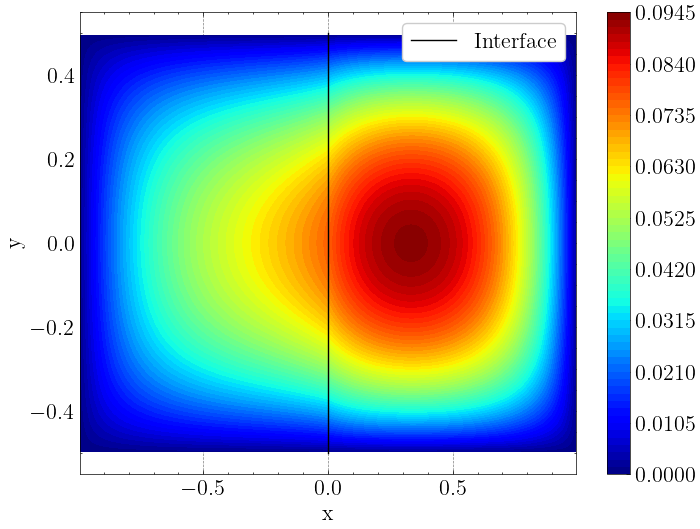
\includegraphics[width=0.9\linewidth]{Images/Transmission/Rectangle_contour_600_150_k1_2.png}
      \caption{Numerical simulation with \(k_1=2\).}
      \label{transmission_rectangle_plot_k1_2}
    \end{minipage}
    
    \vspace{0.5cm} % Add some vertical space between the rows of figures
    
    \begin{minipage}{.6\textwidth}
      \centering
      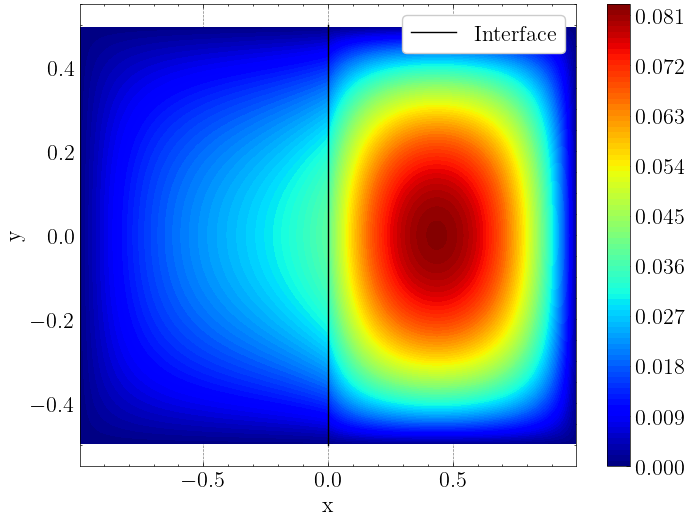
\includegraphics[width=0.8\linewidth]{Images/Transmission/Rectangle_contour_600_150_k1_5.png}
      \caption{Numerical simulation with  \(k_1=5\).}
      \label{transmission_rectangle_plot_k1_5}
    \end{minipage}
    
    \caption*{Numerical approximations of the \ac{BVP} for a rectangular domain with different \(k_1\) values.}
    \label{transmission_rectangle_plots}
\end{figure}

\begin{table}[htbp]
    \centering
    \begin{tabular}{cccccc}
      \toprule
      \multirow{2}{*}{\textbf{\(k_1\) value}} & \multicolumn{2}{c}{\textbf{Boundary Error}} & \multicolumn{2}{c}{\textbf{Interface Errors}} & \multirow{2}{*}{\textbf{Condition number}} \\
      \cmidrule(lr){2-3} \cmidrule(lr){4-5}
      & \textbf{Domain 1} & \textbf{Domain 2} & \textbf{\(e_\gamma^0\)} & \textbf{\(e_\gamma^1\)} & \\
      \midrule
      1 & $7.775\times10^{-8}$ & $7.779\times10^{-8}$ & $4.732\times10^{-9}$ & $7.589\times10^{-9}$ & $2.331\times 10^{13}$\\
      2 & $4.398\times10^{-8}$ & $8.614\times10^{-8}$ & $2.499\times10^{-6}$ & $7.868\times10^{-8}$ & $3.623\times 10^{13}$\\
      5 & $2.181\times10^{-8}$ & $1.036\times10^{-7}$ & $3.838\times10^{-6}$ & $1.551\times10^{-7}$ & $8.182\times 10^{13}$\\
      \bottomrule
    \end{tabular}
    \caption{Consistency errors on the boundary and at the interface \(\gamma\).}
    \label{tab:transmission_results_rectangle}
\end{table}

Figures \ref{transmission_rectangle_plot_k1_1}, \ref{transmission_rectangle_plot_k1_2}, and \ref{transmission_rectangle_plot_k1_5} display the numerical approximations for different \(k_1\) values. Notice that as \(k_1\) increases, the symmetry of the solution is disrupted, causing a shift from \(\Omega_1\) (the left domain) to \(\Omega_2\) (the right domain). Although these results are slightly less accurate than the previous ones due to reduced domain regularity, they still maintain a high level of accuracy. It's worth mentioning that when \(k_1\) and \(k_2\) have different values, the method's accuracy decreases, as expected, since the material parameter changes at the interface, reducing the solution's regularity.

Notice that the condition number of the coefficient matrix \(A\) in \eqref{MFS_transmission_classical_matrices_system} for the rectangle is smaller than the one presented in Table \ref{tab:transmission_results_2} for the unit disk. This is a consequence of a smaller value of \(\eta\) (we recall that in this section we took \(\eta=0.08\) and in the numerical validation section \(\eta=0.3\)), which in this case appears to be optimal since increasing its value decreases the overall accuracy.

\subsection{Results for an L-shape domain with basis functions enrichment}

In the previous subsection, a domain with corners was analyzed. However, it still preserved some regularity, and the \ac{MFS} with classical basis functions was able to capture the behavior of the solution around the corners, for more details on the corner behavior, see Remark \ref{particular_solutions} in Appendix \ref{chapter:appendixB}. In this subsection, we are going to study the case of an L-shaped, nonconvex domain with less regular corners. Two different interfaces will be considered: first, the interface along the line \(x=0\); then, along the symmetry axis of the domain \(\Omega\), i.e. along the line \(y=x+\frac{1}{2}\).

Consider the L-shaped given in Figure \ref{transmission_L_shape_config}. The left and right subdomains are denoted by \(\Omega_1\) and \(\Omega_2\), respectively. The number of interface points is 300, and the number of source points for each domain is 428. The number of boundary collocation points for \(\Omega_1\) and \(\Omega_2\) is 710 and 639, respectively.

\begin{figure}[!htb]
    \centering
    \begin{minipage}{.5\textwidth}
        \centering
        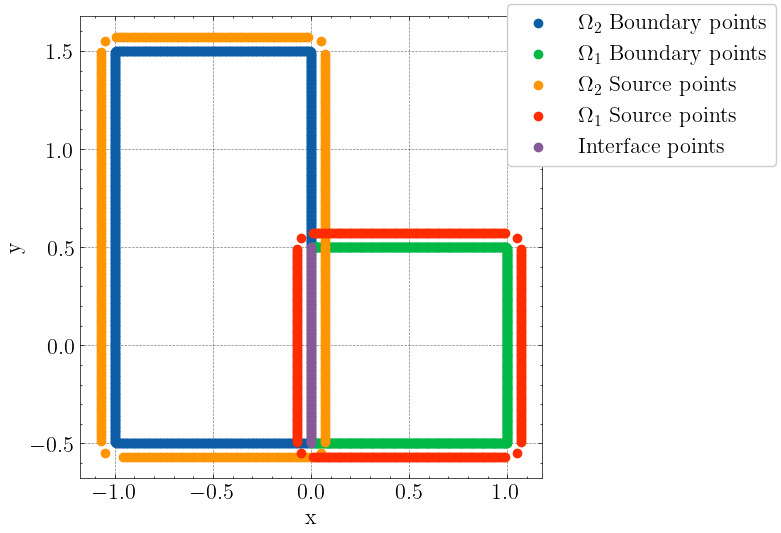
\includegraphics[width=0.75\linewidth]{Images/Transmission/L_shape_2_rectangles_col_points.png}
        \captionsetup{width=0.95\linewidth} % Adjust the width of the caption
        \caption{L-shaped domain with a vertical interface. Configuration of the boundary, source, and interface points.}
        \label{transmission_L_shape_config}
    \end{minipage}%
    %\hspace{0.2cm} % Add some horizontal space between the figures
    \begin{minipage}{.5\textwidth}
        \centering
        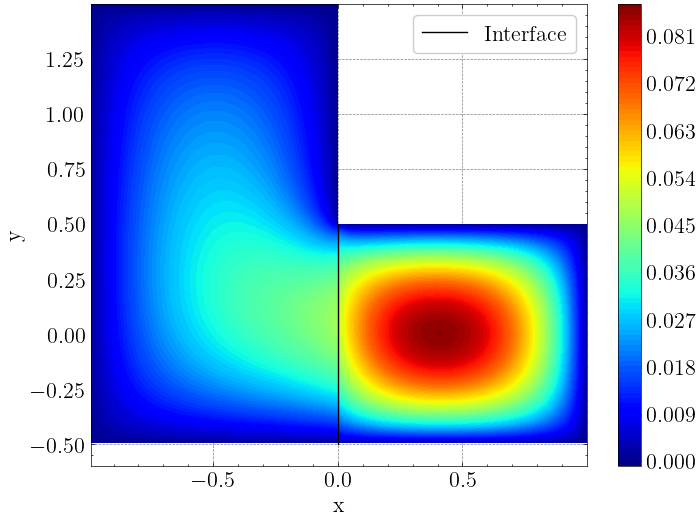
\includegraphics[width=\linewidth]{Images/Transmission/L_shape_2_rectangles_k1_5.png}
        \captionsetup{width=\linewidth} % Adjust the width of the caption
        \caption{Numerical approximation of the transmission problem in an L-shaped domain with interface along \(x=0\) and \(k_1=5\).}
        \label{transmission_L_shape_k1_5}
    \end{minipage}
\end{figure}

In Table \ref{tab:transmission_results_L_shape_rectangles}, the results without resorting to enrichment are presented. It is evident that the method yields poorer results due to the lower regularity of the solution in the re-entrant corner. Particularly, the error along the interface (mainly the lack of continuity) is significantly higher compared to previous cases, even when considering more collocation points on the interface. It appears that the shape of the domain poses more challenges than the discontinuous source function when considering different values for the material parameters \(k_1\) and \(k_2\). In Figure \ref{transmission_L_shape_k1_5}, it is even possible to see that there already exists some small jump near the edges of the interface.

\begin{table}[!htbp]
    \centering
    \begin{tabular}{cccccc}
      \toprule
      \multirow{2}{*}{\textbf{\(k_1\) value}} & \multicolumn{2}{c}{\textbf{Boundary Error}} & \multicolumn{2}{c}{\textbf{Interface Errors}} & \multirow{2}{*}{\textbf{Condition number}} \\
      \cmidrule(lr){2-3} \cmidrule(lr){4-5}
      & \textbf{Domain 1} & \textbf{Domain 2} & \textbf{\(e_\gamma^0\)} & \textbf{\(e_\gamma^1\)} & \\
      \midrule
      1 & $7.853\times10^{-5}$ & $1.155\times10^{-4}$ & $2.916\times10^{-3}$ & $2.155\times10^{-5}$ & $5.587\times 10^{12}$ \\
      2 & $8.152\times10^{-5}$ & $1.350\times10^{-4}$ & $3.835\times10^{-3}$ & $1.149\times10^{-5}$ & $8.161\times 10^{12}$ \\
      5 & $7.079\times10^{-5}$ & $1.378\times10^{-4}$ & $4.085\times10^{-3}$ & $5.411\times10^{-5}$ & $1.776\times 10^{13}$ \\
      \bottomrule
    \end{tabular}
    \caption{Consistency errors on the boundary and in the interface \(\gamma\)}
    \label{tab:transmission_results_L_shape_rectangles}
\end{table}


One of the major problems for the method is the behavior of the solution near the re-entrant corner of \(\Omega\), which in \(\Omega_1\) corresponds to a corner of \(\pi\) radians where different boundary conditions meet (the problem much resembles the \textit{Motz-problem} in \cite{motz1947treatment}, which is used as a benchmark in the study of numerical methods for \acp{PDE} which present singularities, for example in \cite{antunes2010meshfree}).
In this case, we consider Dirichlet-Neumann particular solutions presented in \ref{appendixB_corners} centered in the singular corner. Notice that for \(\Omega_2\) these types of particular solutions are not added to the set of basis functions since the interface edges make a right angle with the adjacent edges.
Therefore, we only consider particular solutions that describe the behavior of the solution in the \(\pi\) radians corner with a possible singularity. Let
\begin{equation}\label{pat_sol_L_shape_rect}
    v_{p_1}(r, \theta) = \beta_{p_1} r^{\alpha_{p_1}} \sin(\beta_{p_1}(\theta - \theta_1))
\end{equation}
where
\[
    \beta_{p_1} = \frac{(p_1+\frac{1}{2})\pi}{\Theta},
\]
\(\theta_1 = \frac{\pi}{2}\), \(\Theta = \pi\) is the total angle amplitude, and where the polar coordinates \(r\) and \(\theta\), centered in the corner, are given by
\[
    r(x,y) = \sqrt{x^2+y^2}, \quad \theta(x,y)=\begin{cases}
        \atantwo(\frac{y}{x}),& \text{if } \atantwo(\frac{y}{x})>0\\
        \atantwo(\frac{y}{x})+2\pi,& \text{if } \atantwo(\frac{y}{x})\leq0,
    \end{cases}
\]
where the function \(\atantwo(y,x)\) computes the \(\arctan\) of \(\frac{y}{x}\) taking into account which quadrant the point \((x, y)\) is in, and it is given by
\[
    \atantwo(y, x) = \begin{cases}
        \arctan(\frac{y}{x}) &\text{ if } x >0,\\
        \arctan(\frac{y}{x}) + \pi &\text{ if } x < 0 \text{ and } y \geq 0,\\
        \atantwo(\frac{y}{x}) -\pi &\text{ if } x < 0 \text{ and } y < 0,\\
        \frac{\pi}{2}, &\text{ if } x = 0 \text{ and } y > 0, \\
        -\frac{\pi}{2}, &\text{ if } x = 0 \text{ and } y < 0, \\
        \text{undefined}, &\text{ if } x = 0 \text{ and } y = 0.
    \end{cases}
\]
See the open standard \cite{jones2010wg14} for more details.
By differentiating Equation \eqref{pat_sol_L_shape_rect} in cartesian coordinates and returning back to polar coordinates we find that
\begin{equation*}
    \nabla v_{p_1}(r, \theta) = \left(-\frac{(2 \pi  {p_1}+\pi )^2 r^{\frac{2 \pi  {p_1}+\pi }{2 \Theta }} \sin \left(\theta +\frac{\pi  \left(p_1+\frac{1}{2}\right) (s-\theta )}{\Theta }\right)}{4 \Theta ^2 r},\frac{(2 \pi  p_1+\pi )^2 r^{\frac{2 \pi  p_1+\pi }{2 \Theta }} \cos \left(\theta +\frac{\pi  \left(p_1+\frac{1}{2}\right) (s-\theta )}{\Theta }\right)}{4 \Theta ^2 r}\right).
\end{equation*}
Finally, considering the truncated expansion
\begin{equation}\label{num_particular_L_shape_rect_equation}
    \phi(r,\theta)=\sum_{p_1=0}^{P_1} \beta_{p_1} v_{p_1}(r, \theta),
\end{equation}
where \(P_1\) is the number of particular solutions added and \(\beta_{p_1}\) are the coefficient to be found using least squares. Expanding the matrix in \eqref{MFS_transmission_classical_matrices_system}, it becomes
\begin{equation}\label{transmission_mat_L_rect_exp}
    \renewcommand{\arraystretch}{1.75} % Increase spacing between rows of the matrices
    \begin{bmatrix}
        \left[\Phi\left(x^{(1)}_{m}-y_j^{(1)}\right)\right] & [0] & \left[\phi(r\left(x_m\right),\theta\left(x_m\right))\right]\\
        [0] & \left[\Phi\left(x^{(2)}_{m}-y_j^{(2)}\right)\right] & \left[0\right]\\
        \left[\Phi\left(z_q-y_j^{(1)}\right)\right] & \left[-\Phi\left(z_q-y_j^{(2)}\right)\right] & \left[\phi(r\left(z_k\right),\theta\left(z_q\right))\right]\\
        \left[k_1\partial_n \Phi\left(z_q-y_j^{(1)}\right)\right] & \left[-k_2 \partial_n \Phi\left(z_q-y_j^{(2)}\right)\right] & \left[k_1 \partial_n\phi(r\left(z_q\right),\theta\left(z_q\right))\right]
    \end{bmatrix}
\end{equation}

Table \ref{tab:transmission_results_L_shape_rectangles_particular} presents the results after applying the enrichment technique for the previously considered \(k_1\) values. In expansion \eqref{num_particular_L_shape_rect_equation}, different numbers of terms were considered. After some simulations, it became clear that choosing \(P_1 > 2\) would not achieve better results for positive \(p_1\) values. On the other hand, negative values of \(p_1\) were considered. Interestingly, when adding particular solutions for the exterior problem, better results were achieved. Not only did the error decrease at the boundary \(\Gamma_i\) of each domain, but better results were also achieved on the interface.

\begin{table}[!htbp]
    \centering
    \begin{longtable}{ccccccc}
        \toprule
        \multicolumn{1}{c}{\textbf{\(p_1\) values}} & \multicolumn{1}{c}{\textbf{\(k_1\) value}} & \multicolumn{2}{c}{\textbf{Boundary Error}} & \multicolumn{2}{c}{\textbf{Interface Errors}} & \multicolumn{1}{c}{\textbf{Condition number}} \\
        \cmidrule(lr){2-2} \cmidrule(lr){3-4} \cmidrule(lr){5-6} \cmidrule(lr){7-7}
        & & \textbf{Domain 1} & \textbf{Domain 2} & \textbf{\(e_\gamma^0\)} & \textbf{\(e_\gamma^1\)} & \\
        \midrule
        \endfirsthead % Header for the first page
        \multicolumn{7}{l}{{\footnotesize\emph{Continued from previous page}}} \\
        \toprule
        \multicolumn{1}{c}{\textbf{\(p\) value}} & \multicolumn{1}{c}{\textbf{\(k_1\) value}} & \multicolumn{2}{c}{\textbf{Boundary Error}} & \multicolumn{2}{c}{\textbf{Interface Errors}} & \multicolumn{1}{c}{\textbf{Condition number}} \\
        \cmidrule(lr){2-2} \cmidrule(lr){3-4} \cmidrule(lr){5-6} \cmidrule(lr){7-7}
        & & \textbf{Domain 1} & \textbf{Domain 2} & \textbf{\(C^0\)} & \textbf{\(C^1\)} & \\
        \midrule
        \endhead % Header for subsequent pages
        \midrule[\heavyrulewidth] % Horizontal line
        \multicolumn{7}{r}{{\footnotesize\emph{Continued on next page}}} \\
        \endfoot % Footer for subsequent pages
        \bottomrule
        \endlastfoot % Footer for the last page
        
        % Data for p = [0, 1]
        0, 1 & 1 & $2.965\times10^{-5}$ & $7.907\times10^{-5}$ & $2.94\times10^{-3}$ & $2.624\times10^{-5}$ & $5.584\times10^{12}$ \\
        & 2 & $2.203\times10^{-5}$ & $6.657\times10^{-5}$ & $1.86\times10^{-3}$ & $2.068\times10^{-5}$ & $8.156\times10^{12}$ \\
        & 5 & $2.203\times10^{-5}$ & $6.657\times10^{-5}$ & $1.86\times10^{-3}$ & $2.068\times10^{-5}$ & $8.156\times10^{12}$ \\
        \midrule[\heavyrulewidth] % Horizontal line
        
        % Data for p = [-1, 0, 1]
        -1, 0, 1 & 1 & $8.627\times10^{-6}$ & $4.132\times10^{-5}$ & $7.68\times10^{-4}$ & $6.876\times10^{-6}$ & $5.585\times10^{12}$ \\
        & 2 & $7.333\times10^{-6}$ & $2.791\times10^{-5}$ & $6.01\times10^{-4}$ & $2.555\times10^{-5}$ & $8.157\times10^{12}$ \\
        & 5 & $4.271\times10^{-6}$ & $1.118\times10^{-5}$ & $2.69\times10^{-4}$ & $4.166\times10^{-5}$ & $1.775\times10^{13}$ \\
        \midrule[\heavyrulewidth] % Horizontal line

        % Data for p = [-2, -1, 0, 1]
        -2, -1, 0, 1 & 1 & $3.898\times10^{-6}$ & $5.975\times10^{-6}$ & $1.44\times10^{-3}$ & $2.505\times10^{-6}$ & $4.156\times10^{14}$ \\
        & 2 & $2.584\times10^{-6}$ & $2.514\times10^{-6}$ & $9.69\times10^{-4}$ & $1.048\times10^{-5}$ & $4.156\times10^{14}$ \\
        & 5 & $1.119\times10^{-6}$ & $6.838\times10^{-7}$ & $4.89\times10^{-4}$ & $1.106\times10^{-5}$ & $4.156\times10^{14}$ \\
        \midrule[\heavyrulewidth] % Horizontal line
    \end{longtable}
    \caption{Consistency errors on the boundary and at the interface \(\gamma\) after enriching the basis with particular (angular) solutions}
    \label{tab:transmission_results_L_shape_rectangles_particular}
\end{table}

To finish this subsection, we present an L-shaped domain where the interface is drawn along its axis of symmetry. In this case, notice that there are two singular corners, both with \(\frac{3}{4}\pi\) radians\footnote{The other two corners have an angle of \(\frac{\pi}{4}\) radians which cause no problem for the classical \ac{MFS} basis functions.}. In Figure \ref{transmission_L_shape_col_axis_config}, we present the configuration with \(\Omega_1\) extending further up and \(\Omega_2\) further right. The number of interface points and source points for each domain is still 300 and 428, respectively. We also chose 628 boundary collocation points for both domains. Table \ref{tab:transmission_results_L_shape_axis} summarizes the results without considering particular solutions.

\begin{figure}[!htb]
    \centering
    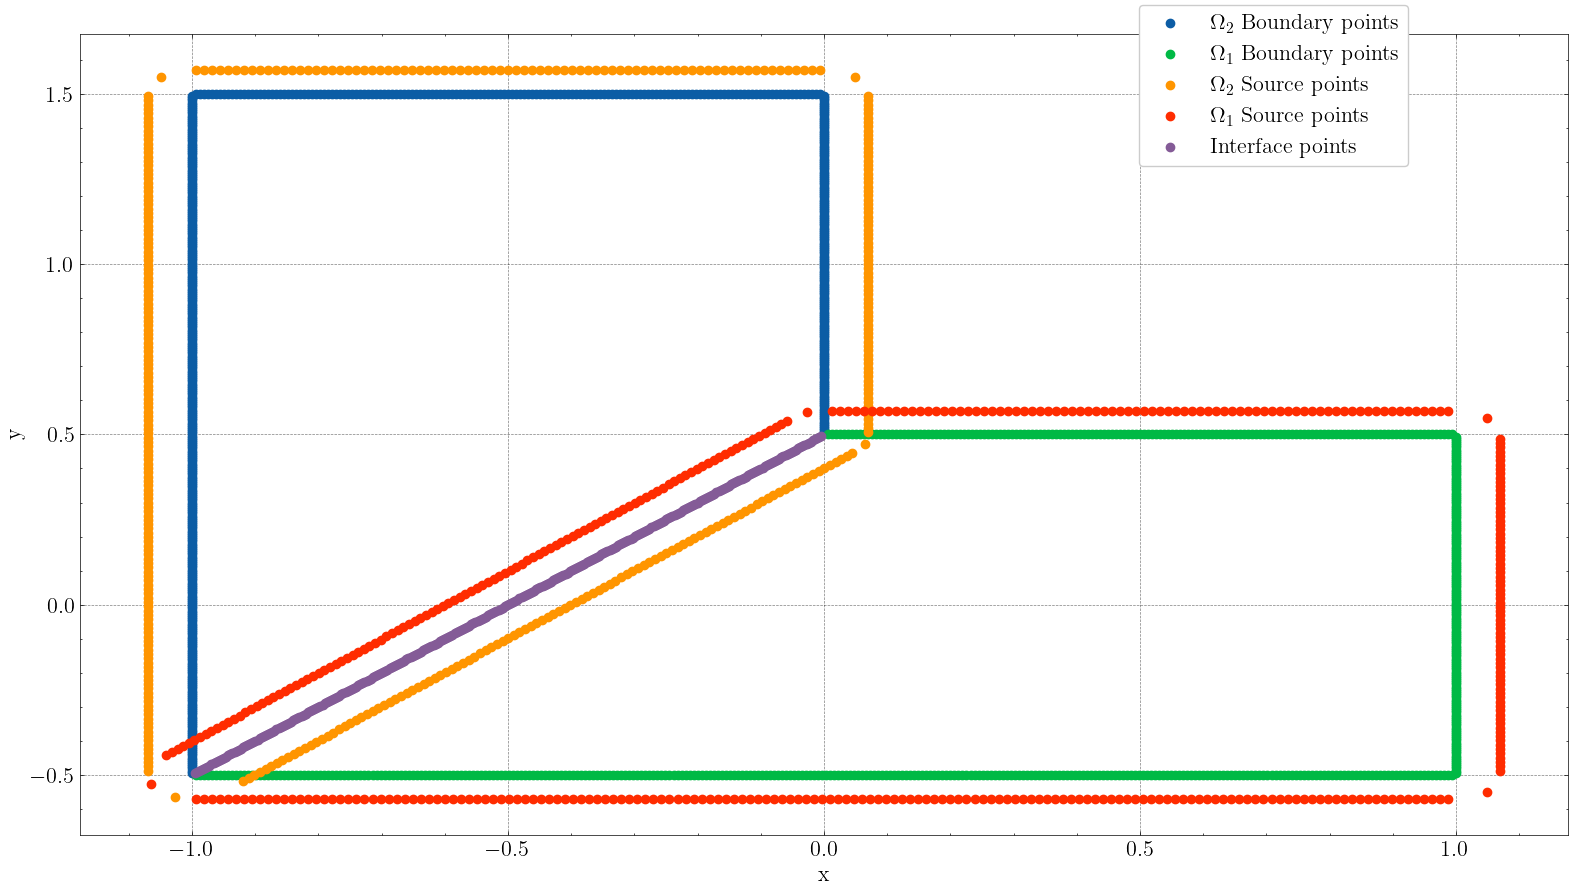
\includegraphics[height=0.38\linewidth,width=0.5\linewidth]{Images/Transmission/L_shape_2_axis_col_points.png}
    %\captionsetup{width=0.9\linewidth} % Adjust the width of the caption
    \caption{L-shaped domain with the interface on the symmetry axis. Configuration of the boundary, source, and interface points.}
    \label{transmission_L_shape_col_axis_config}
\end{figure}

\begin{table}[!htbp]
    \centering
    \begin{tabular}{cccccc}
      \toprule
      \multirow{2}{*}{\textbf{\(k_1\) value}} & \multicolumn{2}{c}{\textbf{Boundary Error}} & \multicolumn{2}{c}{\textbf{Interface Errors}} & \multirow{2}{*}{\textbf{Condition number}} \\
      \cmidrule(lr){2-3} \cmidrule(lr){4-5}
      & \textbf{Domain 1} & \textbf{Domain 2} & \textbf{\(e_\gamma^0\)} & \textbf{\(e_\gamma^1\)} & \\
      \midrule
      1 & $1.812\times10^{-4}$ & $2.060\times10^{-4}$ & $7.305\times10^{-3}$ & $8.018\times10^{-5}$ & $1.050\times 10^{10}$ \\
      2 & $1.398\times10^{-4}$ & $9.729\times10^{-5}$ & $5.986\times10^{-4}$ & $5.505\times10^{-5}$ & $1.646\times 10^{10}$ \\
      5 & $7.096\times10^{-5}$ & $3.030\times10^{-5}$ & $1.528\times10^{-3}$ & $4.348\times10^{-5}$ & $3.730\times 10^{10}$ \\
      \bottomrule
    \end{tabular}
    \caption{Consistency errors on the boundary and at the interface \(\gamma\)}
    \label{tab:transmission_results_L_shape_axis}
\end{table}

Since particular solutions will be added at the singular corners in \(\Omega_2\), one should now consider Neumann-Dirichlet particular solutions centered in the singular corner (check section \ref{appendixB_corners} in Appendix \ref{chapter:appendixB} for more details). These particular solutions have the form
\[
    w_{p_2}(r,\theta) = \beta_{p_2} r^{\beta_{p_2}}\cos(\beta_{p_2}(\theta-\theta_2)),
\]
where the \(\beta_{p_2}\) coefficients are the same as in \eqref{pat_sol_L_shape_rect}, \(\Theta = \frac{3}{4}\pi\) and \(\theta_2=\frac{5}{4}\pi\). Notice that \(\Theta\) is the same in both domains. The (polar) gradient of \(w\) is now
\begin{equation*}
    \nabla w(r,\theta)_{p_2} = \left(\frac{(2 \pi  {p_2}+\pi )^2 r^{\frac{2 \pi  {p_2}+\pi }{2 \Theta }} \cos \left(\theta +\frac{\pi  \left({p_2}+\frac{1}{2}\right) (s-\theta )}{\Theta }\right)}{4 \Theta ^2 r},\frac{(2 \pi  {p_2}+\pi )^2 r^{\frac{2 \pi  {p_2}+\pi }{2 \Theta }} \sin \left(\theta +\frac{\pi  \left({p_2}+\frac{1}{2}\right) (s-\theta )}{\Theta }\right)}{4 \Theta ^2 r}\right).
\end{equation*}

Table \ref{tab:transmission_results_L_shape_axis_particular} shows the results obtained when particular solutions are added to both domains. Once again, negative values of \(p_2\) were considered. Without intending to show too much data (because we would have to account for every combination of \(p_1\) and \(p_2\) values), we fix \(p_2=0, 1\). The reason for this choice is that better results are achieved when increasing the number of particular solutions in the domain where the diffusion coefficient is higher. Since we are only varying \(k_1\), we can fix the \(p_2\) values.
%\vspace*{1.1cm}
\pagebreak
\begin{table}[!htbp]
    \centering
    \begin{longtable}{ccccccc}
        \toprule
        \multicolumn{1}{c}{\textbf{\(p_1\) values}} & \multicolumn{1}{c}{\textbf{\(k_1\) value}} & \multicolumn{2}{c}{\textbf{Boundary Error}} & \multicolumn{2}{c}{\textbf{Interface Errors}} & \multicolumn{1}{c}{\textbf{Condition number}} \\
        \cmidrule(lr){2-2} \cmidrule(lr){3-4} \cmidrule(lr){5-6} \cmidrule(lr){7-7}
        & & \textbf{Domain 1} & \textbf{Domain 2} & \textbf{\(e_\gamma^0\)} & \textbf{\(e_\gamma^1\)} & \\
        \midrule
        \endfirsthead % Header for the first page
        \multicolumn{7}{l}{{\footnotesize\emph{Continued from previous page}}} \\
        \toprule
        \multicolumn{1}{c}{\textbf{\(p\) value}} & \multicolumn{1}{c}{\textbf{\(k_1\) value}} & \multicolumn{2}{c}{\textbf{Boundary Error}} & \multicolumn{2}{c}{\textbf{Interface Errors}} & \multicolumn{1}{c}{\textbf{Condition number}} \\
        \cmidrule(lr){2-2} \cmidrule(lr){3-4} \cmidrule(lr){5-6} \cmidrule(lr){7-7}
        & & \textbf{Domain 1} & \textbf{Domain 2} & \textbf{\(C^0\)} & \textbf{\(C^1\)} & \\
        \midrule
        \endhead % Header for subsequent pages
        \midrule[\heavyrulewidth] % Horizontal line
        \multicolumn{7}{r}{{\footnotesize\emph{Continued on next page}}} \\
        \endfoot % Footer for subsequent pages
        \bottomrule
        \endlastfoot % Footer for the last page
        
        % Data for p = [0, 1]
        0, 1 & 1 & $3.107\times10^{-7}$ & $2.100\times10^{-7}$ & $1.158\times10^{-5}$ & $1.019\times10^{-7}$ & $1.054\times10^{10}$ \\
        & 2 & $1.061\times10^{-7}$ & $6.892\times10^{-7}$ & $6.366\times10^{-5}$ & $7.065\times10^{-8}$ & $1.648\times10^{10}$ \\
        & 5 & $1.207\times10^{-7}$ & $1.141\times10^{-6}$ & $9.544\times10^{-5}$ & $9.487\times10^{-8}$ & $3.732\times10^{10}$ \\
        \midrule[\heavyrulewidth] % Horizontal line
        
        % Data for p = [-1, 0, 1]
        -1, 0, 1 & 1 & $3.319\times10^{-7}$ & $2.026\times10^{-7}$ & $1.813\times10^{-5}$ & $1.048\times10^{-7}$ & $1.054\times10^{10}$ \\
        & 2 & $1.676\times10^{-7}$ & $3.166\times10^{-7}$ & $8.375\times10^{-6}$ & $7.951\times10^{-8}$ & $1.647\times10^{10}$ \\
        & 5 & $9.871\times10^{-8}$ & $4.807\times10^{-7}$ & $1.549\times10^{-6}$ & $5.285\times10^{-8}$ & $3.732\times10^{10}$ \\
        \midrule[\heavyrulewidth] % Horizontal line

        % Data for p = [-2, -1, 0, 1]
        -2, -1, 0, 1 & 1 & $3.070\times10^{-7}$ & $2.415\times10^{-7}$ & $1.610\times10^{-5}$ & $9.893\times10^{-8}$ & $5.659\times10^{12}$ \\
        & 2 & $1.762\times10^{-7}$ & $2.670\times10^{-7}$ & $8.385\times10^{-6}$ & $8.480\times10^{-8}$ & $5.656\times10^{12}$ \\
        & 5 & $9.761\times10^{-8}$ & $3.201\times10^{-7}$ & $1.993\times10^{-6}$ & $6.049\times10^{-8}$ & $5.655\times10^{12}$ \\
        \midrule[\heavyrulewidth] % Horizontal line
    \end{longtable}
    \caption{Consistency errors on the boundary and at the interface \(\gamma\) after adding particular (angular) solutions to the classical \ac{MFS} basis.}
    \label{tab:transmission_results_L_shape_axis_particular}
\end{table}

% \begin{longtable}{ccccccc}
%         \caption{Numerical relative error on the boundary and in the interface \(\gamma\) after considering particular (angular) solutions}
%         \label{tab:transmission_results_L_shape_axis_particular}
%         \toprule
%         \multicolumn{1}{c}{\textbf{\(p_1\) values}} & \multicolumn{1}{c}{\textbf{\(k_1\) value}} & \multicolumn{2}{c}{\textbf{Boundary Error}} & \multicolumn{2}{c}{\textbf{Interface Errors}} & \multicolumn{1}{c}{\textbf{Condition number}} \\
%         \cmidrule(lr){2-2} \cmidrule(lr){3-4} \cmidrule(lr){5-6} \cmidrule(lr){7-7}
%         & & \textbf{Domain 1} & \textbf{Domain 2} & \textbf{\(C^0\)} & \textbf{\(C^1\)} & \\
%         \midrule
%         \endfirsthead % Header for the first page
%         \multicolumn{7}{l}{{\footnotesize\emph{Continued from previous page}}} \\
%         \toprule
%         \multicolumn{1}{c}{\textbf{\(p\) value}} & \multicolumn{1}{c}{\textbf{\(k_1\) value}} & \multicolumn{2}{c}{\textbf{Boundary Error}} & \multicolumn{2}{c}{\textbf{Interface Errors}} & \multicolumn{1}{c}{\textbf{Condition number}} \\
%         \cmidrule(lr){2-2} \cmidrule(lr){3-4} \cmidrule(lr){5-6} \cmidrule(lr){7-7}
%         & & \textbf{Domain 1} & \textbf{Domain 2} & \textbf{\(C^0\)} & \textbf{\(C^1\)} & \\
%         \midrule
%         \endhead % Header for subsequent pages
%         \midrule[\heavyrulewidth] % Horizontal line
%         \multicolumn{7}{r}{{\footnotesize\emph{Continued on next page}}} \\
%         \endfoot % Footer for subsequent pages
%         \bottomrule
%         \endlastfoot % Footer for the last page
        
%         % Data for p = [0, 1]
%         0, 1 & 1 & $3.107\times10^{-7}$ & $2.100\times10^{-7}$ & $1.158\times10^{-5}$ & $1.019\times10^{-7}$ & $1.054\times10^{10}$ \\
%         & 2 & $1.061\times10^{-7}$ & $6.892\times10^{-7}$ & $6.366\times10^{-5}$ & $7.065\times10^{-8}$ & $1.648\times10^{10}$ \\
%         & 5 & $1.207\times10^{-7}$ & $1.141\times10^{-6}$ & $9.544\times10^{-5}$ & $9.487\times10^{-8}$ & $3.732\times10^{10}$ \\
%         \midrule[\heavyrulewidth] % Horizontal line
        
%         % Data for p = [-1, 0, 1]
%         -1, 0, 1 & 1 & $3.319\times10^{-7}$ & $2.026\times10^{-7}$ & $1.813\times10^{-5}$ & $1.048\times10^{-7}$ & $1.054\times10^{10}$ \\
%         & 2 & $1.676\times10^{-7}$ & $3.166\times10^{-7}$ & $8.375\times10^{-6}$ & $7.951\times10^{-8}$ & $1.647\times10^{10}$ \\
%         & 5 & $9.871\times10^{-8}$ & $4.807\times10^{-7}$ & $1.549\times10^{-6}$ & $5.285\times10^{-8}$ & $3.732\times10^{10}$ \\
%         \midrule[\heavyrulewidth] % Horizontal line

%         % Data for p = [-2, -1, 0, 1]
%         -2, -1, 0, 1 & 1 & $3.070\times10^{-7}$ & $2.415\times10^{-7}$ & $1.610\times10^{-5}$ & $9.893\times10^{-8}$ & $5.659\times10^{12}$ \\
%         & 2 & $1.762\times10^{-7}$ & $2.670\times10^{-7}$ & $8.385\times10^{-6}$ & $8.480\times10^{-8}$ & $5.656\times10^{12}$ \\
%         & 5 & $9.761\times10^{-8}$ & $3.201\times10^{-7}$ & $1.993\times10^{-6}$ & $6.049\times10^{-8}$ & $5.655\times10^{12}$ \\
%         \midrule[\heavyrulewidth] % Horizontal line
% \end{longtable}


%\vspace*{2cm}

Again, we found the same surprising results as before, that is, with negative values for \(p_1\) we achieve better approximations, particularly when \(k_1 \neq k_2 = 1\). An interesting observation was made when both \(p_1\) and \(p_2\) had negative values. In that case, the numerical solution exploded in both domains. Intuitively, it seems that one cannot consider singular functions everywhere around a corner. On the other hand, one may consider \(p_1 = p_2 = 0, \dots, P\), where \(P=P_1=P_2\), for \(P > 1\) (\(P\) may be as large as 8, for example, with 16 particular solutions being added in total) and the results can be as good as the ones presented in Table \ref{tab:transmission_results_L_shape_axis_particular} for \(p_1=-2, -1, 0, 1\), but only if \(k_1=k_2=1\); otherwise, the approximation on the interface gets worse. 

\begin{figure}[!htb]
    \centering
    \begin{minipage}{.5\textwidth}
      \centering
      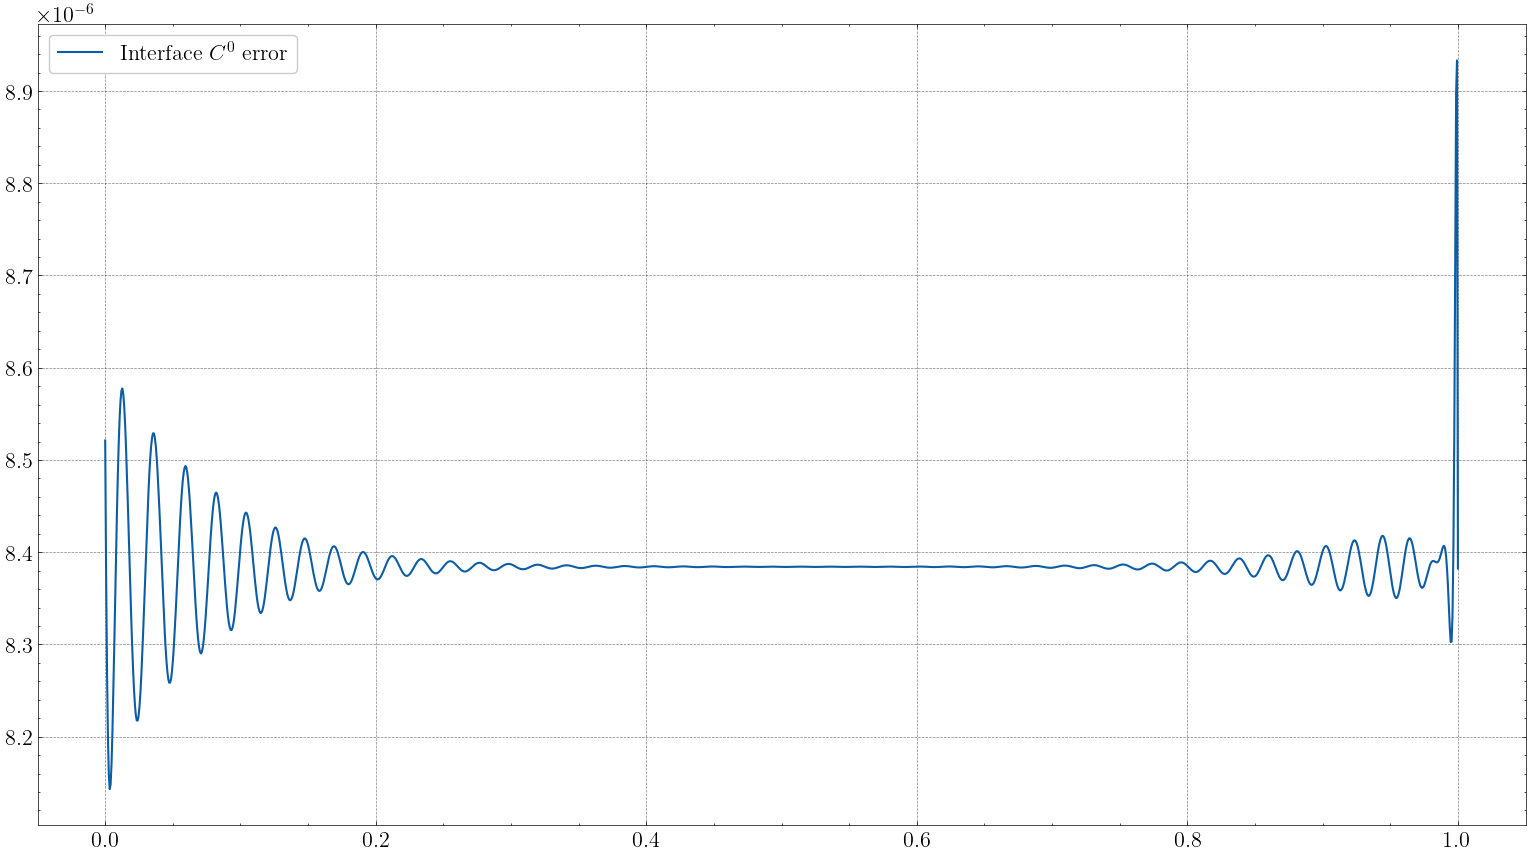
\includegraphics[width=1\linewidth]{Images/Transmission/L_shape_2_axis_c0_error_k1_2_enr.png}
      \caption{Interface \(C^0\) error}
      \label{transmission_L_axis_error_c0_k1_2}
    \end{minipage}%
    \begin{minipage}{.5\textwidth}
      \centering
      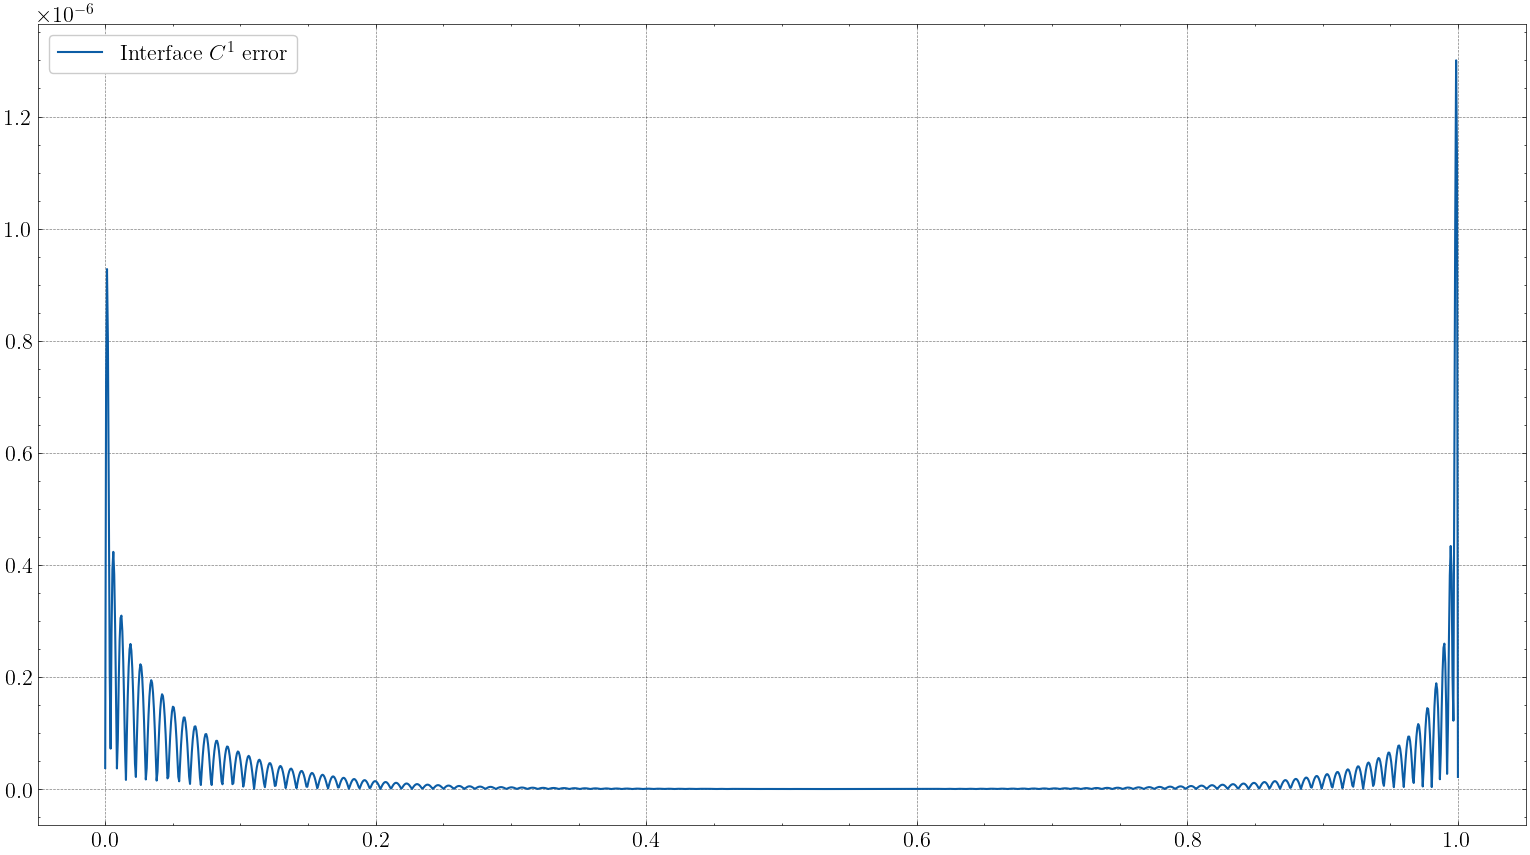
\includegraphics[width=1\linewidth]{Images/Transmission/L_shape_2_axis_c1_error_k1_2_enr.png}
      \caption{Interface \(C^0\) error}
      \label{transmission_L_axis_error_c1_k1_2}
    \end{minipage}
    
    \vspace{0.5cm} % Add some vertical space between the rows of figures
    
    \begin{minipage}{.6\textwidth}
      \centering
      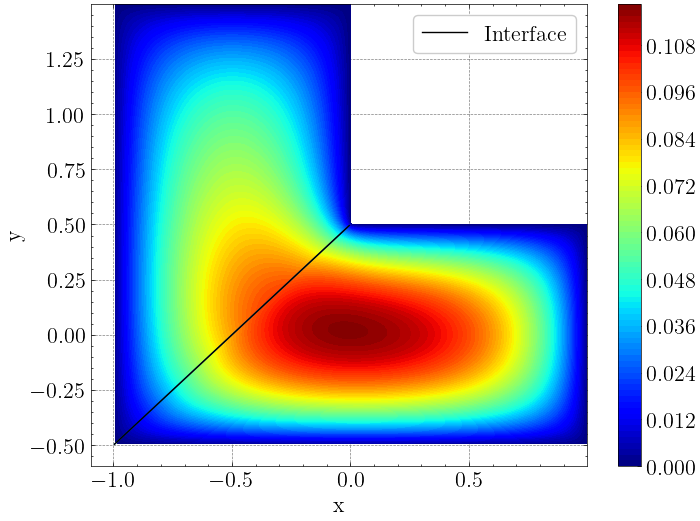
\includegraphics[width=\linewidth]{Images/Transmission/L_shape_2_axis_sol_k1_2_enr.png}
      %\caption{Numerical approximation}
      \label{transmission_L_axis_plot_k1_2}
    \end{minipage}
    
    \caption{Absolute value of the interface errors and numerical approximation for \(k_1=2\), \(p_1=-2, -1, 0, 1\) and \(p_2 = 0, 1\).}
    \label{}
\end{figure}

Figures \ref{transmission_L_axis_error_c0_k1_2} and \ref{transmission_L_axis_error_c1_k1_2} show the absolute value of the errors for each interface point, with \(k_1=2\) and the \(p\) values for the particular solutions are \(p_1=-2, -1, 0, 1\) and \(p_2 = 0, 1\). As expected, both errors peak near the endpoints of the interface, in particular near the singular corner.